\documentclass{article}

% --- Bộ mã và font tiếng Việt ---
\usepackage[utf8]{inputenc}
\usepackage[T5]{fontenc}
\usepackage[vietnamese]{babel}

% --- Hình ảnh và đồ họa ---
\usepackage{amsmath}
\usepackage{graphicx}
\usepackage{amssymb}
\usepackage{tcolorbox}
\tcbuselibrary{skins}
\usepackage{fontawesome5} 
\usepackage{enumitem}
\usepackage{float}
\usepackage{subcaption}
\usepackage{tikz}
\usetikzlibrary{arrows.meta, positioning, shapes.geometric, arrows}

% --- Trình bày văn bản ---
\usepackage[outputdir=.]{minted}
\usepackage{caption}
\usepackage{fancybox}
\usepackage{titlesec}
\usepackage{tabularx} 
\usepackage{tocloft}
\usepackage{listings}
\usepackage{xcolor}
\usepackage{lipsum}
\usepackage{array}
\usepackage{ulem}
\usepackage{fancyhdr}
\usepackage[top=3.0cm, bottom=3.0cm, left=3.0cm, right=2.0cm, a4paper, margin=2cm]{geometry}
\usepackage{indentfirst}
\usepackage{setspace}
\onehalfspacing

% --- Định nghĩa các biến ---
\definecolor{codegreen}{rgb}{0,0.6,0}
\definecolor{codegray}{rgb}{0.5,0.5,0.5}
\definecolor{codepurple}{rgb}{0.58,0,0.82}
\definecolor{backcolour}{rgb}{0.95,0.95,0.92}

% --- Định nghĩa văn bản dạng code ---
\lstdefinestyle{asm}{
    backgroundcolor=\color{backcolour},   
    commentstyle=\color{codegreen},
    keywordstyle=\color{magenta},
    numberstyle=\tiny\color{codegray},
    stringstyle=\color{codepurple},
    basicstyle=\ttfamily\footnotesize,
    breakatwhitespace=false,         
    breaklines=true,                 
    captionpos=b,                    
    keepspaces=true,                 
    numbers=left,                    
    numbersep=5pt,                  
    showspaces=false,                
    showstringspaces=false,
    showtabs=false,                  
    tabsize=4,
    frame=single,
    language=[x86masm]Assembler
}

% --- Định nghĩa style Flowchart ---
\tikzstyle{startstop} = [rectangle, rounded corners, minimum width=3cm, minimum height=1cm,text centered, draw=black, fill=red!30]
\tikzstyle{process} = [rectangle, minimum width=3cm, minimum height=1cm, text centered, draw=black, fill=blue!20]
\tikzstyle{decision} = [diamond, minimum width=3cm, minimum height=1cm, text centered, draw=black, fill=yellow!30]
\tikzstyle{arrow} = [thick,->,>=stealth]

% --- Header & Footer ---
\pagestyle{fancy}
\fancyhf{}
\fancyhead[L]{Bài tập lớn KIẾN TRÚC MÁY TÍNH}
\fancyhead[R]{Triệu Tuấn Anh - B23DCCN053}
\fancyfoot[C]{\thepage}

% --- Hyperlink cho mục lục ---
\usepackage[hidelinks]{hyperref}

\setlength{\cftbeforesecskip}{5pt} % Khoảng cách giữa các mục \section
\setlength{\cftbeforesubsecskip}{5pt} % Khoảng cách giữa các mục \subsection

% --- Định nghĩa danh sách code (tương tự list of figures) ---
\newcommand{\listofcodename}{\LARGE \bfseries DANH SÁCH MÃ NGUỒN}
\newcommand{\listofcode}{\large \listof{lstlisting}{\listofcodename}}

\begin{document}

% --- Trang bìa ---
\begin{titlepage}
\begin{tikzpicture}[remember picture, overlay]
% --- Viền ngoài ---
\draw[line width=2pt, rounded corners=10pt]
    ([shift={(1cm,-1cm)}] current page.north west)
    rectangle
    ([shift={(-1cm,1cm)}] current page.south east);
% --- Viền trong ---
\draw[line width=1pt, rounded corners=8pt]
    ([shift={(1.5cm,-1.5cm)}] current page.north west)
    rectangle
    ([shift={(-1.5cm,1.5cm)}] current page.south east);
\end{tikzpicture}

\begin{center}
\vspace*{1.2cm}

% --- Trường và khoa ---
{\bfseries\Large HỌC VIỆN CÔNG NGHỆ BƯU CHÍNH VIỄN THÔNG}\\[0.4cm]
{\bfseries\large KHOA CÔNG NGHỆ THÔNG TIN}

\vspace{0.5cm}
\noindent\rule{0.85\textwidth}{0.8pt}
\vspace{1cm}

% --- Logo ---

\includegraphics[width=5cm]{Images/logo.png}
\vspace{1.5cm}

% --- Tiêu đề ---
{\bfseries\fontsize{24}{28}\selectfont BÀI TẬP LỚN}\\[0.5cm]
{\bfseries\fontsize{20}{24}\selectfont MÔN: KIẾN TRÚC MÁY TÍNH}

\vspace{2cm}

% --- Thông tin sinh viên ---
\begin{center}
\begin{tcolorbox}[colframe=black!80, colback=white, boxrule=0.8pt, arc=6pt, width=0.75\textwidth]
{\setstretch{1.5}
\noindent
\begin{tabular}{@{}l l@{}}
\textbf{\large Họ và tên:} & {\large Triệu Tuấn Anh} \\
\textbf{\large Mã sinh viên:} & {\large B23DCCN053} \\
\textbf{\large Lớp:} & {\large D23CQCN11-B} \\
\textbf{\large Giảng viên hướng dẫn:} & {\large Trần Tiến Công} \\
\end{tabular}
}
\end{tcolorbox}
\end{center}

\vspace*{\fill}

% --- Dòng cuối ---
{\bfseries\fontsize{14}{18}\selectfont Hà Nội, 2025}

\end{center}
\end{titlepage}

\newpage

% --- Mục lục ---
\renewcommand{\contentsname}{\centering \LARGE \bfseries MỤC LỤC}
\tableofcontents
\thispagestyle{empty} % Không đánh số trang ở mục lục

\vspace{1cm}
\vspace*{\fill}
\noindent\rule{\textwidth}{0.4pt} % Đường kẻ dưới mục lục

% --- Danh sách hình ảnh ---
\newpage
\thispagestyle{empty}
\renewcommand{\listfigurename}{\centering \LARGE \bfseries DANH SÁCH HÌNH ẢNH}
\listoffigures
\newpage

% --- Danh sách mã nguồn ---
\newpage
\thispagestyle{empty}
\listofcode
\newpage

% --- Nội dung ---
\section{Phần cá nhân}
\subsection{Bài số 1: Lập trình hợp ngữ Assembly}
% --- Câu 1 ---
\subsubsection{\textit{Câu 1}}

\noindent\textbf{\large Đề bài:} Viết chương trình hợp ngữ Assembly cho phép nhập vào một số và in ra màn hình giai thừa của số đó.

\vspace{0.5cm}
\noindent\textbf{\large Biểu diễn bằng Flowchart:} hình \ref{fig:flowchart-1}

\begin{figure}[H]
    \centering
    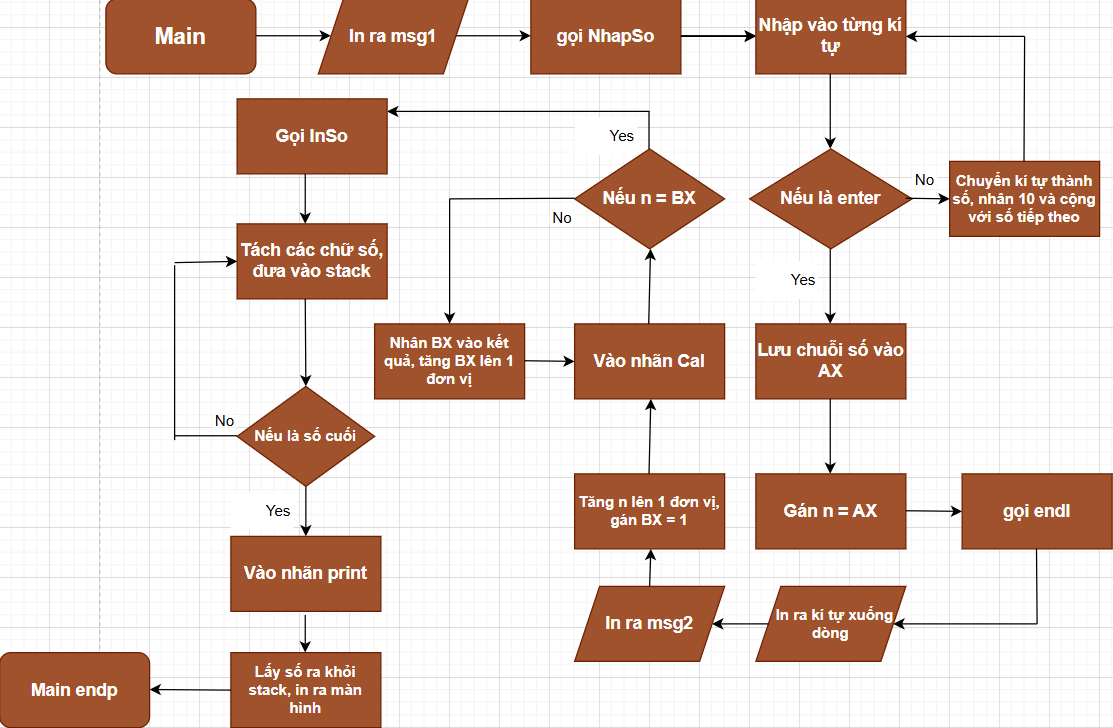
\includegraphics[width=1\textwidth]{Images/Flowchart/Flowchart-1.png}
    \caption{Flowchart tính giai thừa 1 số}
    \label{fig:flowchart-1}
\end{figure}

\vspace{0.5cm}
\noindent\textbf{\large Mã nguồn assembly 8086:}
\begin{lstlisting}[style=asm, caption={Mã nguồn câu 1}]
    .model small               ;Khoi tao che do bo nho la small
    .stack 100                 ;Khoi tao kich thuoc ngan xep
    .data                      ;Khoi tao cac bien
        crlf db 13, 10, '$'      
        x dw ?
        y dw ? 
        n dw ? 
        msg1 db 'Nhap vao 1 so: $'
        msg2 db 'Giai thua cua so da nhap la: $'
    .code
    main proc                  ;Ham chinh cua chuong trinh
        mov ax, @data
        mov ds, ax             ;Khoi tao thanh ghi ds
        
        mov ah, 9              ;In ra msg1
        lea dx, msg1
        int 21h
        
        call NhapSo            ;Thuc hien nhap so
        mov n, ax              ;Luu so vua nhap vao n
        call endl              ;Xuong dong
        
        mov ah, 9              ;In ra msg2
        lea dx, msg2
        int 21h
        
        inc n                  ;Tang n len 1 don vi
        mov bx, 1              ;Khoi tao thanh ghi bx
        mov ax, 1              ;Khoi tao thanh ghi ax de luu ket qua
        Cal:
            cmp bx, n          ;So sanh bx voi n
            je break           ;Neu bx = n thi thuc hien break
            mul bx             ;Neu bx != n thi nhan ax voi bx, luu vao ax
            inc bx             ;Tang bx len 1 don vi
            jmp Cal            ;Tiep tuc lap de tinh giai thua
        break:
        call InSo              ;In ra ket qua
        
        mov ah, 4ch            ;Ket thuc chuong trinh
        int 21h
    main endp 
    
    NhapSo proc                ;Ham con de nhap so
        mov x, 0               ;Khoi tao x = 0
        mov y, 0               ;Khoi tao y = 0
        mov bx, 10             ;Khoi tao bx = 10
        nhap:   
            mov ah, 1          ;Nhap 1 ki tu
            int 21h 
            cmp al, 13         ;Neu ki tu la dau enter thi chay vao nhapxong
            je nhapxong
            sub al, '0'        ;Neu ki tu khong phai enter thi bien doi thanh so
            mov ah, 0
            mov y, ax          ;Luu so vua nhap vao y
            mov ax, x
            mul bx             ;Lay ax * bx, ket qua luu vao ax
            add ax, y          ;Lay ax + y, ket qua luu vao ax
            mov x, ax          
            jmp nhap           ;Tiep tuc lap den khi nhap xong
        nhapxong:
            mov ax, x          ;Luu so da nhap vao thanh ghi ax
        ret
    NhapSo endp 
    
    endl proc                   ;Ham con de xuong dong
        push ax
        push dx
        
        mov ah, 9               ;In ra ki tu xuong dong
        lea dx, crlf
        int 21h
        
        pop dx
        pop ax
        ret
    endl endp  
    
    InSo proc                  ;Ham con de in so
        push ax
        push bx
        push cx
        push dx
        
        mov bx, 10             ;Khoi tao bx = 10
        mov cx, 0              ;Khoi tao cx = 0
        beforePrint:
            mov dx, 0
            div bx             ;Thuc hien ax / bx, phan nguyen luu vao ax, phan du luu vao dx
            push dx            ;Day phan du vao ngan xep
            inc cx             ;Tang cx 
            cmp ax, 0          ;Neu ax > 0 thi tiep tuc tach so
            jg beforePrint
        print:
            pop dx             ;Lap phan du ra khoi ngan xep
            mov ah, 2          
            add dx, '0'        ;Bien doi so thanh ki tu
            int 21h            ;In ra man hinh
            loop print         ;Lap cho den khi in xong
        
        pop dx
        pop cx
        pop bx
        pop ax
        ret
    InSo endp
    
    end main
\end{lstlisting}

\vspace{0.5cm}
\noindent\textbf{\large Giao diện hiển thị: } hình \ref{fig:result-1}

\begin{figure}[H]
    \centering
    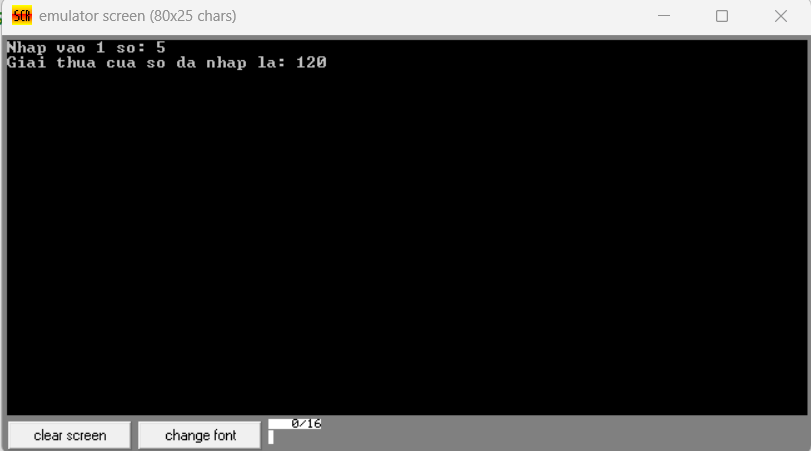
\includegraphics[width=0.8\textwidth]{Images/Result/B1.png}
    \caption{Giao diện hiển thị câu 1}
    \label{fig:result-1}
\end{figure}

% --- Câu 2 ---
\subsubsection{\textit{Câu 2}}

\noindent\textbf{\large Đề bài:} Viết chương trình hợp ngữ cho phép nhập vào một mảng gồm 10 số có hai chữ số. Tính tổng các số chia hết cho 7. In tổng thu được ra màn hình dưới dạng thập phân.

\vspace{0.5cm}
\noindent\textbf{\large Biểu diễn bằng Flowchart:} hình \ref{fig:flowchart-2}

\begin{figure}[H]
    \centering
    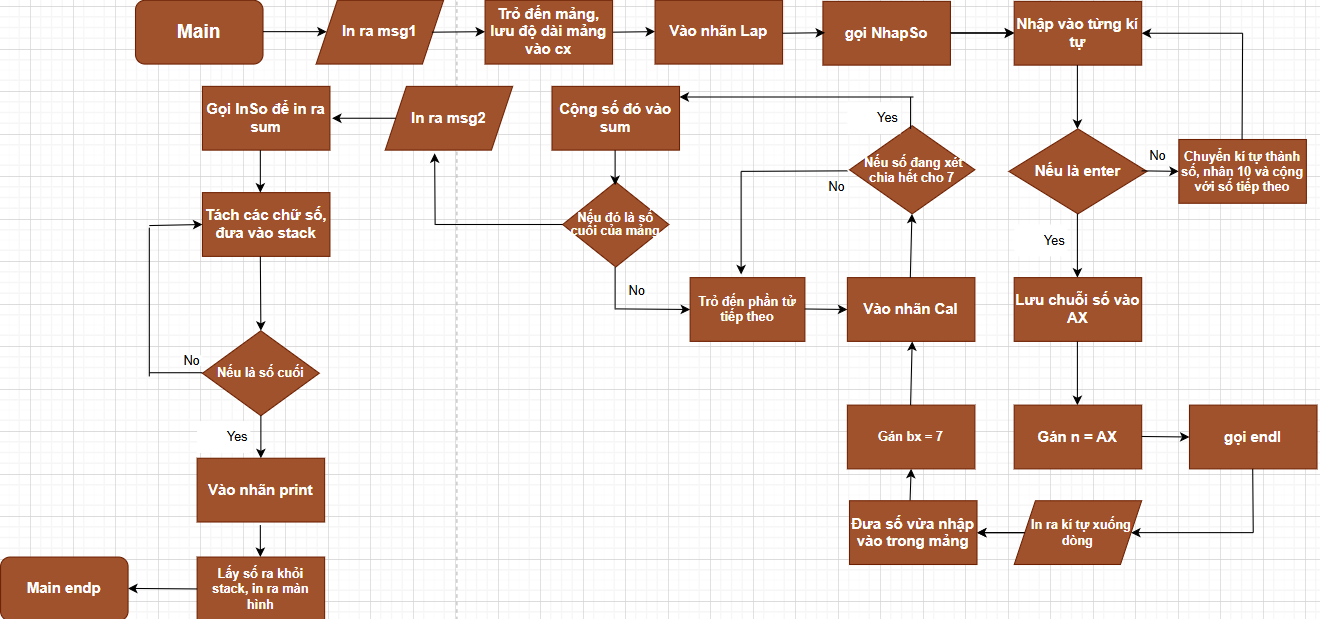
\includegraphics[width=1\textwidth]{Images/Flowchart/Flowchart-2.png}
    \caption{Flowchart tính tổng số chia hết cho 7}
    \label{fig:flowchart-2}
\end{figure}

\vspace{0.5cm}
\noindent\textbf{\large Mã nguồn assembly 8086:}
\begin{lstlisting}[style=asm, caption={Mã nguồn câu 2}]
    .model small               ;Khoi tao che do bo nho la small
    .stack 100                 ;Khoi tao kich thuoc ngan xep
    .data                      ;Khoi tao cac bien
        crlf db 13, 10, '$'                
        x dw ?
        y dw ?              
        sum dw ?
        arr dw 10 dup('$')
        msg1 db 'Nhap 10 so co 2 chu so (moi so tren 1 dong):', 0Dh, 0Ah, '$'
        msg2 db 'Tong cac so chia het cho 7 la: $'
    .code
    main proc                  ;Ham chinh cua chuong trinh
        mov ax, @data
        mov ds, ax             ;Khoi tao thanh ghi ds
        
        mov ah, 9              ;In ra man hinh msg1
        lea dx, msg1
        int 21h
        
        lea si, arr            ;Thanh ghi SI tro den mang arr
        mov cx, 10             ;Luu do dai arr vao thanh ghi cx
        Lap:
            call NhapSo  
            call endl
            mov [si], ax       ;Dua moi so nhap duoc vao trong mang arr
            add si, 2          ;Tang SI tro den phan tu tiep theo cua mang, vi mang dw nen phai +2
            loop Lap           ;Thuc hien nhap mang cho den khi du phan tu
        
        mov cx, 10             ;Luu do dai arr vao thanh ghi cx
        lea si, arr            ;Thanh ghi SI tro den mang arr
        mov bx, 7              ;Luu 7 vao thanh ghi bx 
        Cal:
            mov dx, 0          ;Gan thanh dx = 0
            mov ax, [si]       ;Lay ra tung phan tu dua vao thanh ax
            div bx             ;Lay ax chia bx, phan nguyen luu vao ax, phan du luu vao dx
            cmp dx, 0          ;So sanh dx voi 0
            jne continue       ;Neu dx != 0 thi nhay den continue
            mov ax, [si]       ;Neu dx == 0, tuc la chia het cho 7
            add sum, ax        ;Neu chia het cho 7 thi cong vao sum
            continue:
            add si, 2          ;Tang si tro den phan tu tiep theo
            loop Cal           ;Thuc hien so sanh den phan tu cuoi cung cua mang
        
        mov ah, 9              ;In ra msg2
        lea dx, msg2
        int 21h 
        
        mov ax, sum            ;Dua gia tri cua sum vao thanh ghi ax
        call InSo              ;In ra ket qua
        mov ah, 4ch            ;Ket thuc chuong trinh
        int 21h
    main endp 
    
    NhapSo proc                ;Ham con de nhap so
        mov x, 0               ;Khoi tao x = 0
        mov y, 0               ;Khoi tao y = 0
        mov bx, 10             ;Khoi tao bx = 10
        nhap:   
            mov ah, 1          ;Nhap 1 ki tu
            int 21h 
            cmp al, 13         ;Neu ki tu la dau enter thi chay vao nhapxong
            je nhapxong
            sub al, '0'        ;Neu ki tu khong phai enter thi bien doi thanh so
            mov ah, 0
            mov y, ax          ;Luu so vua nhap vao y
            mov ax, x
            mul bx             ;Lay ax * bx, ket qua luu vao ax
            add ax, y          ;Lay ax + y, ket qua luu vao ax
            mov x, ax          
            jmp nhap           ;Tiep tuc lap den khi nhap xong
        nhapxong:
            mov ax, x          ;Luu so da nhap vao thanh ghi ax
        ret
    NhapSo endp 
    
    endl proc                   ;Ham con de xuong dong
        push ax
        push dx
        
        mov ah, 9               ;In ra ki tu xuong dong
        lea dx, crlf
        int 21h
        
        pop dx
        pop ax
        ret
    endl endp  
    
    InSo proc                  ;Ham con de in so
        push ax
        push bx
        push cx
        push dx
        
        mov bx, 10             ;Khoi tao bx = 10
        mov cx, 0              ;Khoi tao cx = 0
        beforePrint:
            mov dx, 0
            div bx             ;Thuc hien ax / bx, phan nguyen luu vao ax, phan du luu vao dx
            push dx            ;Day phan du vao ngan xep
            inc cx             ;Tang cx 
            cmp ax, 0          ;Neu ax > 0 thi tiep tuc tach so
            jg beforePrint
        print:
            pop dx             ;Lap phan du ra khoi ngan xep
            mov ah, 2          
            add dx, '0'        ;Bien doi so thanh ki tu
            int 21h            ;In ra man hinh
            loop print         ;Lap cho den khi in xong
        
        pop dx
        pop cx
        pop bx
        pop ax
        ret
    InSo endp
    
    end main
\end{lstlisting}

\vspace{0.5cm}
\noindent\textbf{\large Giao diện hiển thị: } hình \ref{fig:result-2}

\begin{figure}[H]
    \centering
    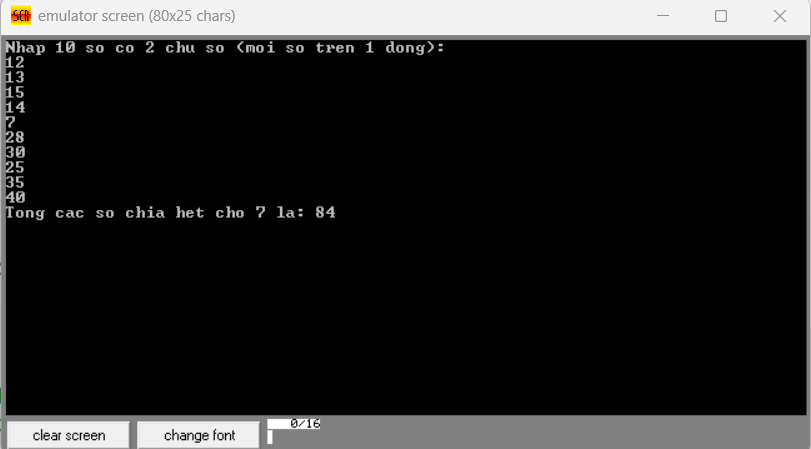
\includegraphics[width=0.8\textwidth]{Images/Result/B2.png}
    \caption{Giao diện hiển thị câu 2}
    \label{fig:result-2}
\end{figure}



% --- Câu 3 ---
\subsubsection{\textit{Câu 3}}

\noindent\textbf{\large Đề bài:} Viết chương trình hợp ngữ cho hai chuỗi ký tự A và B có độ dài là n và m (n > m), chỉ ra xâu B có phải là xâu con của xâu A không? Nếu xâu B là xâu con của xâu A thì chỉ ra vị trí xâu B ở xâu A.

\vspace{0.5cm}
\noindent\textbf{\large Biểu diễn bằng Flowchart:} hình \ref{fig:flowchart-3}

\begin{figure}[H]
    \centering
    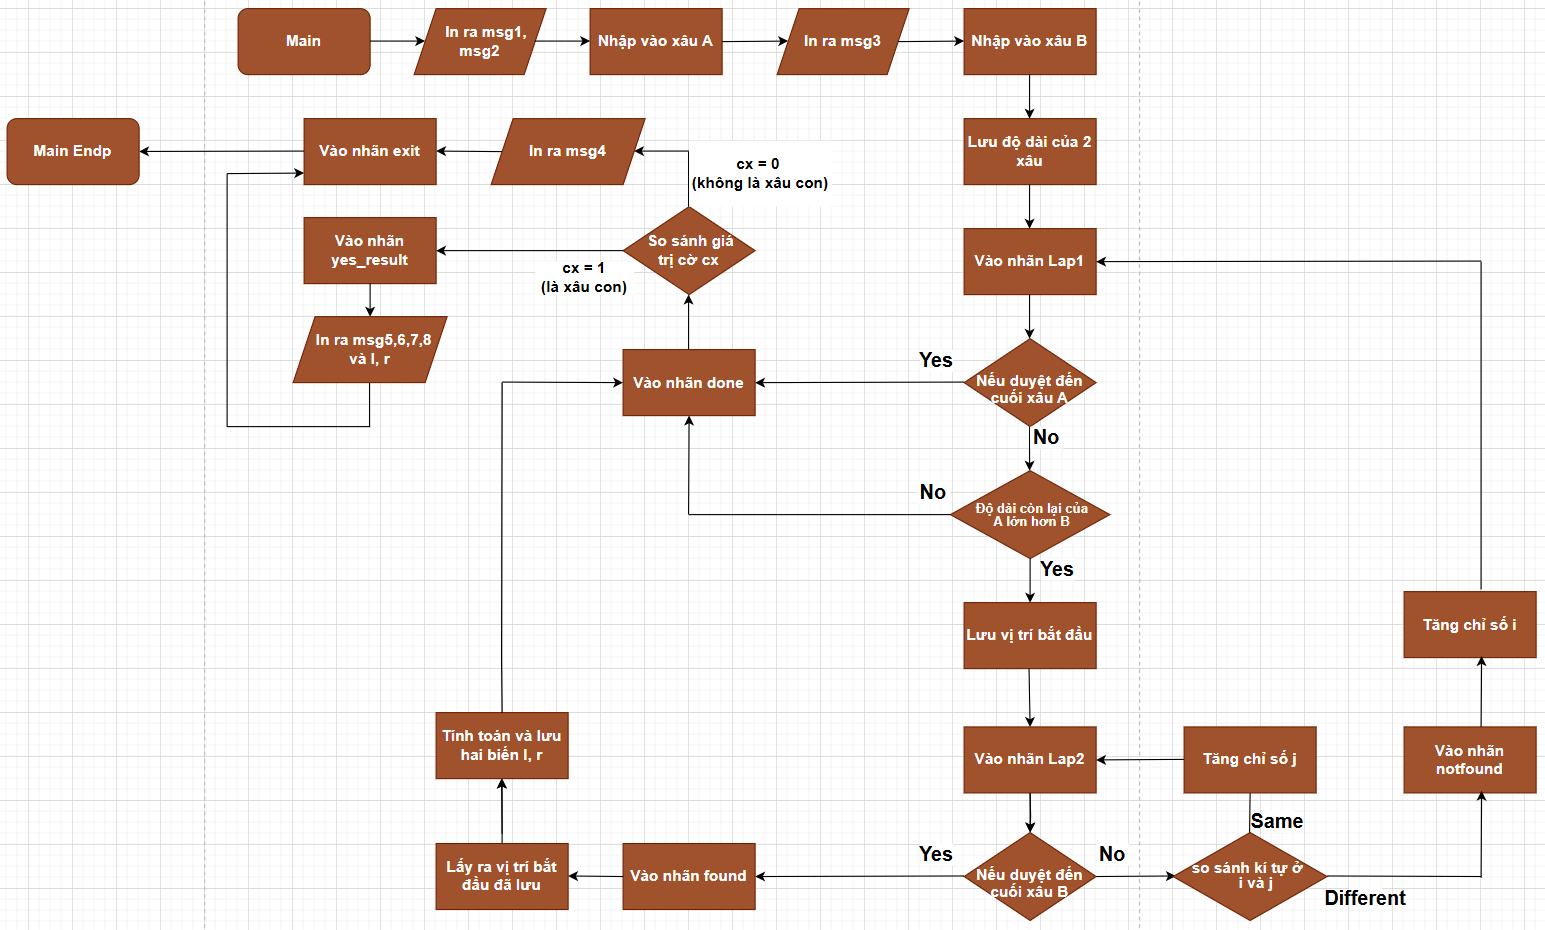
\includegraphics[width=1\textwidth]{Images/Flowchart/Flowchart-3.png}
    \caption{Flowchart kiểm tra xâu con}
    \label{fig:flowchart-3}
\end{figure}

\vspace{0.5cm}
\noindent\textbf{\large Mã nguồn assembly 8086:}
\begin{lstlisting}[style=asm, caption={Mã nguồn câu 3}]
    .model small
    .stack 100
    .data
        crlf db 13, 10, '$'      
        msg1 db 'Nhap vao 2 xau A, B (luu y xau A dai hon xau B)$'
        msg2 db 'Nhap vao xau A: $'
        msg3 db 'Nhap vao xau B: $'
        msg4 db 'B khong la xau con cua A$'      
        msg5 db 'B la xau con cua A$'
        msg6 db 'Vi tri cua B: $'    
        msg7 db 'Tu ki tu $'
        msg8 db ' den ki tu $'
        l dw ?
        r dw ?
        strA db 50, ?, 50 dup('$')
        strB db 50, ?, 50 dup('$')
        lenA db ?
        lenB db ?
    
    .code
    main proc
        mov ax, @data
        mov ds, ax
    
        mov ah, 9                 ;In ra msg1
        lea dx, msg1
        int 21h
        call endl
    
        mov ah, 9                 ;In ra msg2
        lea dx, msg2
        int 21h    
        
        mov ah, 10
        lea dx, strA              ;Nhap xau A
        int 21h
        call endl
    
        mov ah, 9                 ;In ra msg3
        lea dx, msg3
        int 21h      
        
        mov ah, 10                ;Nhap xau B
        lea dx, strB
        int 21h
        call endl
    
        mov al, [strA + 1]        ;Luu do dai strA vao lenA
        mov lenA, al
        mov al, [strB + 1]        ;Luu do dai strB vao lenB
        mov lenB, al                          
        
        lea si, strA + 2           ;si tro vao dau xau A
        mov cx, 0                  ;cx = 0 => chua tim thay
        mov dl, 0                  ;Chi so i trong A
    
        Lap1:
            cmp dl, lenA              ;Neu i >= lenA thi lap xong
            jnl done                   
            mov al, lenA              
            sub al, dl
            cmp al, lenB
            jb done                   ;Phan con lai < do dai B => khong the co xau con
        
            push si                   ;Luu vi tri bat dau
            lea di, strB + 2          ;di tro vao xau B
            mov dh, 0                 ;Chi so j trong B
            mov bx, si                ;bx tro vao vi tri so sanh trong A
        
        Lap2:
            cmp dh, lenB              ;Neu j chay den het strB thi thoa man la xau con
            je found
            mov al, [bx]              ;So sanh chi so i va j
            cmp al, [di]
            jne notfound              ;Neu i != j thi vao nhan not_found
            inc bx                    ;Neu i == j thi tang i, j
            inc di
            inc dh
            jmp Lap2
        
        found:
            pop si                    ;Lay ra vi tri bat dau
            mov cx, 1                 ;cx = 1 => da tim thay
            mov ax, si
            sub ax, offset strA + 2   ;Tinh toan vi tri bat dau
            inc ax                    ;Tang ax vi bat dau tinh tu vi tri 1
            mov l, ax                 ;Luu gia tri vao l
            mov ax, l
            mov bl, lenB              ;Lay vi tri dau tien cong voi
            add ax, bx                ;do dai strB de ra vi tri cuoi cung
            dec ax
            mov r, ax                 ;Luu gia tri vao r
            jmp done
        
        notfound:
            pop si                    ;Neu khong tim thay, tro den vi tri tiep theo trong strA
            inc si
            inc dl
            jmp Lap1
        
        done:
            cmp cx, 1                 ;So sanh cx voi 1 
            je yes_result             ;Neu cx = 1 => vao nhan yes_result
        
            mov ah, 9                 ;Neu cx = 0 => in ra msg4
            lea dx, msg4
            int 21h
            jmp exit
        
        yes_result:
            mov ah, 9                 ;In ra msg5
            lea dx, msg5
            int 21h
            call endl
        
            mov ah, 9                 ;In ra msg6
            lea dx, msg6
            int 21h
        
            mov ah, 9                 ;In ra msg7
            lea dx, msg7
            int 21h
        
            mov ax, l                 ;In ra l
            call InSo
        
            mov ah, 9                 ;In ra msg8
            lea dx, msg8
            int 21h
        
            mov ax, r                 ;In ra r
            call InSo
        
        exit:
        mov ah, 4ch
        int 21h
    main endp
    
    endl proc
        push ax
        push dx
        mov ah, 9
        lea dx, crlf           ;In ra ki tu xuong dong
        int 21h
        pop dx
        pop ax
        ret
    endl endp
    
    InSo proc                       ;Ham in so nguyen
        push ax
        push bx
        push cx
        push dx
    
        mov bx, 10
        mov cx, 0
        next_digit:
            mov dx, 0
            div bx
            push dx
            inc cx
            cmp ax, 0
            jg next_digit
    
        print_digits:
            pop dx
            add dl, '0'
            mov ah, 2
            int 21h
            loop print_digits
    
        pop dx
        pop cx
        pop bx
        pop ax
        ret
    InSo endp
    
    end main
\end{lstlisting}

\vspace{0.5cm}
\noindent\textbf{\large Giao diện hiển thị: } hình \ref{fig:result-3-1} và hình \ref{fig:result-3-2}

\begin{figure}[H]
    \centering
    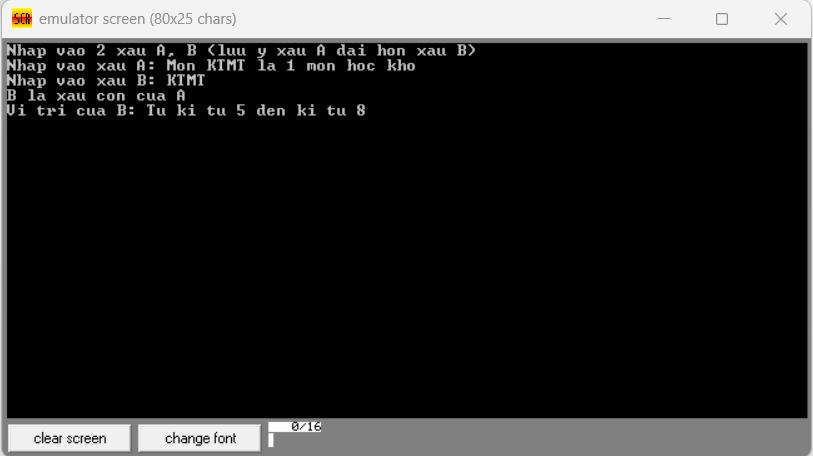
\includegraphics[width=0.8\textwidth]{Images/Result/B3-1.png}
    \caption{Giao diện hiển thị câu 3 - Trường hợp hợp lệ}
    \label{fig:result-3-1}
\end{figure}

\begin{figure}[H]
    \centering
    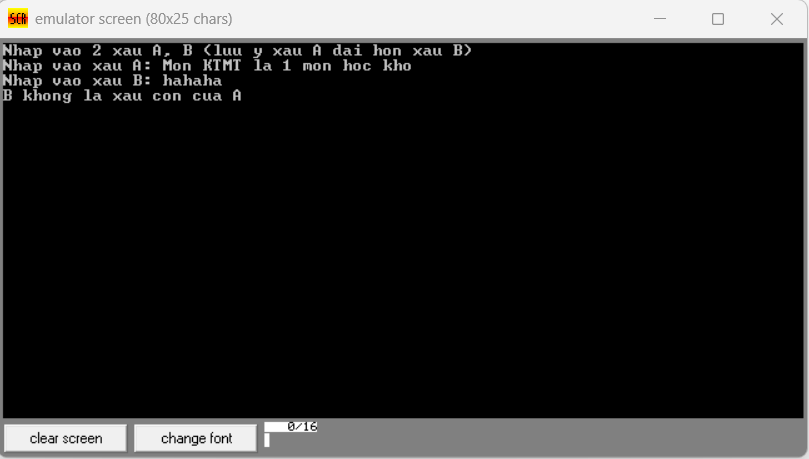
\includegraphics[width=0.8\textwidth]{Images/Result/B3-2.png}
    \caption{Giao diện hiển thị câu 3 - Trường hợp không hợp lệ}
    \label{fig:result-3-2}
\end{figure}



\subsection{Bài số 2: Thực hành phân tích khảo sát hệ thống bộ nhớ}
% --- Subtask 1 ---
\subsubsection{\textit{Khảo sát cấu hình của máy và hệ thống bộ nhớ của máy đang sử dụng (Bộ nhớ trong: ROM, RAM, Cache System; Bộ nhớ ngoài: ổ đĩa cứng, CD, Thiết bị vào ra)}}

\noindent\textbf{\large Phần mềm khảo sát:} 
\begin{itemize}
    \item Sử dụng phần mềm CPU-Z 64-bit Ver. 2.15
    \item Sử dụng các chương trình quản lí đĩa và thiết bị trên máy tính (Disk Management và Device Manager)
\end{itemize}

\vspace{0.5cm}

% --- CPU ---
\noindent\textbf{\large CPU:} (Thông số chi tiết thể hiện ở Hình \ref{fig:cpu-z-cpu})

\begin{itemize}
    \item \textbf{Tên CPU:} Intel Core i3-10110U
    \item \textbf{Kiến trúc:} Comet Lake-U/Y
    \item \textbf{Tiến trình sản xuất:} 14nm
    \item \textbf{TDP tối đa:} 15W (rất tiết kiệm điện, phù hợp cho laptop)
    \item \textbf{Socket:} 1528 FCBGA (dạng hàn chết lên mainboard, phổ biến ở laptop)
    \item \textbf{Số nhân - Số luồng:} 2 nhân, 4 luồng
    \item \textbf{Xung nhịp cơ bản:} 2.10 GHz (thể hiện ở dòng "Specification")
    \item \textbf{Xung nhịp hiện tại:} Khoảng 900 MHz
    \item \textbf{Bus Speed:} 100.35 MHz
    \item \textbf{Tập lệnh hỗ trợ:} MMX, SSE (và các biến thể), AVX, AVX2, FMA3,...
\end{itemize}

\begin{center}
    \fbox{\parbox{0.9\textwidth}{
        \centering
        \large Đây là một CPU tiết kiệm điện, phổ biến trên các laptop mỏng nhẹ, hiệu năng vừa đủ cho các tác vụ văn phòng, học tập, hoặc giải trí nhẹ nhàng.
    }}
\end{center}

\begin{figure}[H]
    \centering
    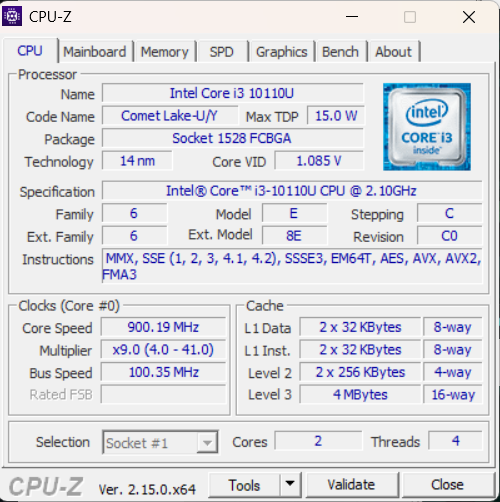
\includegraphics[width=0.75\textwidth]{Images/Stats/CPU.png}
    \caption{Giao diện phần mềm CPU-Z - Tab CPU}
    \label{fig:cpu-z-cpu}
\end{figure}

% --- Cache ---
\noindent\textbf{\large Cache:} (Thông số chi tiết thể hiện ở Hình \ref{fig:cpu-z-cache})

\begin{itemize}
    \item \textbf{L1 Cache (Level 1 Cache):}
    \begin{itemize}
        \item \textbf{Data:} 2 × 32 KB
        \item \textbf{Instruction:} 2 × 32 KB
        \item \textbf{Tổ chức:} 8-way associative (8 đường liên kết)
        \item \textit{Ghi chú:} Đây là bộ nhớ cache nhanh nhất và nhỏ nhất, chia riêng biệt cho dữ liệu và lệnh. Mỗi nhân có cache riêng.
    \end{itemize}
    
    \item \textbf{L2 Cache (Level 2 Cache):}
    \begin{itemize}
        \item \textbf{Dung lượng:} 2 × 256 KB
        \item \textbf{Tổ chức:} 4-way associative
        \item \textit{Ghi chú:} Mỗi nhân có 256 KB cache L2 riêng biệt, trung gian giữa L1 và L3.
    \end{itemize}
    
    \item \textbf{L3 Cache (Level 3 Cache):}
    \begin{itemize}
        \item \textbf{Dung lượng:} 4 MB (chia sẻ giữa các nhân)
        \item \textbf{Tổ chức:} 16-way associative
        \item \textit{Ghi chú:} Đây là cache lớn nhất và được chia sẻ chung cho tất cả các nhân CPU, giúp giảm độ trễ khi trao đổi dữ liệu giữa các nhân.
    \end{itemize}
\end{itemize}

\begin{center}
    \fbox{\parbox{0.9\textwidth}{
        \centering
        \large Cache cấp thấp hơn (L1) thì nhỏ nhưng cực nhanh, trong khi cấp cao hơn (L3) thì lớn hơn nhưng tốc độ chậm hơn. Cấu trúc nhiều cấp như vậy giúp tối ưu tốc độ truy xuất bộ nhớ của CPU.
    }}
\end{center}

\begin{figure}[H]
    \centering
    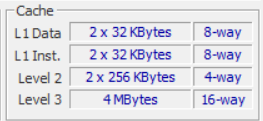
\includegraphics[width=0.5\textwidth]{Images/Stats/Cache.png}
    \caption{Giao diện phần mềm CPU-Z - Bộ nhớ Cache}
    \label{fig:cpu-z-cache}
\end{figure}

% --- RAM ---
\noindent\textbf{\large RAM:} (Thông số chi tiết thể hiện ở Hình \ref{fig:cpu-z-memory})

\begin{itemize}
    \item \textbf{Loại RAM:} DDR4
    \item \textbf{Dung lượng:} 8 GB
    \item \textbf{Số kênh (Channel):} Dual (2 kênh)
    \item \textbf{Tần số thực tế (DRAM Frequency):} 665.5 MHz
    \item \textbf{Tỉ lệ FSB:DRAM:} 3:20
    \item \textbf{Độ trễ CAS (CL):} 10.0 clocks
    \item \textbf{RAS to CAS Delay (tRCD):} 10 clocks
    \item \textbf{RAS Precharge (tRP):} 10 clocks
    \item \textbf{Cycle Time (tRAS):} 28 clocks
    \item \textbf{Row Refresh Cycle Time (tRFC):} 234 clocks
    \item \textbf{Command Rate (CR):} 1T
\end{itemize}

\begin{center}
    \fbox{\parbox{0.9\textwidth}{
        \centering
        \large RAM của hệ thống này có cấu hình cân bằng, đáp ứng tốt nhu cầu phổ thông, đồng thời nhờ Dual Channel mà hiệu suất cũng khá ổn định và mượt mà trong các tác vụ đa nhiệm.
    }}
\end{center}

\begin{figure}[H]
    \centering
    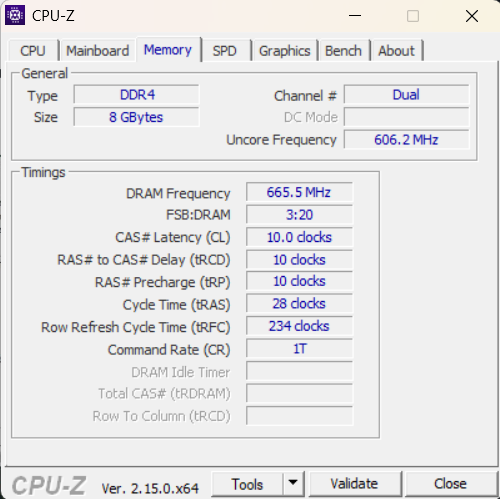
\includegraphics[width=0.5\textwidth]{Images/Stats/Memory.png}
    \caption{Giao diện phần mềm CPU-Z - Bộ nhớ}
    \label{fig:cpu-z-memory}
\end{figure}

% --- Bộ nhớ ngoài ---
\noindent\textbf{\large Bộ nhớ ngoài:} (Thông số chi tiết thể hiện ở Hình \ref{fig:cpu-z-disk})

\begin{itemize}
    \item \textbf{Ổ cứng:} 1 ổ cứng vật lý (Disk 0)
    \item \textbf{Dung lượng tổng:} 238.46 GB
    \item \textbf{Cấu trúc phân vùng:}
    \begin{itemize}
        \item \textbf{OS (C:)} 119.60 GB (NTFS)
        \begin{itemize}
            \item Phân vùng chứa hệ điều hành Windows.
            \item Còn trống: 33.73 GB (khoảng 28\% dung lượng).
        \end{itemize}
        \item \textbf{Data (D:)} 117.19 GB (NTFS)
        \begin{itemize}
            \item Phân vùng lưu trữ dữ liệu cá nhân.
            \item Còn trống: 110.64 GB (khoảng 94\% dung lượng).
        \end{itemize}
        \item \textbf{Phân vùng hệ thống và khôi phục:}
        \begin{itemize}
            \item 260 MB (EFI System Partition) -- phân vùng khởi động.
            \item 1.22 GB (Recovery Partition) -- phân vùng phục hồi hệ thống.\\Dùng để khôi phục máy về trạng thái ban đầu (Factory Reset) như lúc mới mua.
            \item 200 MB (Recovery Partition) -- phân vùng phục hồi hệ thống.\\Dùng để sửa lỗi khởi động (Startup Repair), khôi phục hệ thống (System Restore), reset PC (Reset This PC), hoặc truy cập Command Prompt khi hệ điều hành gặp sự cố.
        \end{itemize}
    \end{itemize}
    \item \textbf{Hệ thống tập tin:} NTFS cho các phân vùng chính.
\end{itemize}

\begin{center}
    \fbox{\parbox{0.9\textwidth}{
        \centering
        \large Ổ đĩa đang được phân vùng hợp lý, tách riêng dữ liệu và hệ điều hành. Dung lượng dữ liệu còn trống nhiều, không có phân vùng lỗi, hệ thống đang vận hành ổn định.
    }}
\end{center}

\begin{figure}[H]
    \centering
    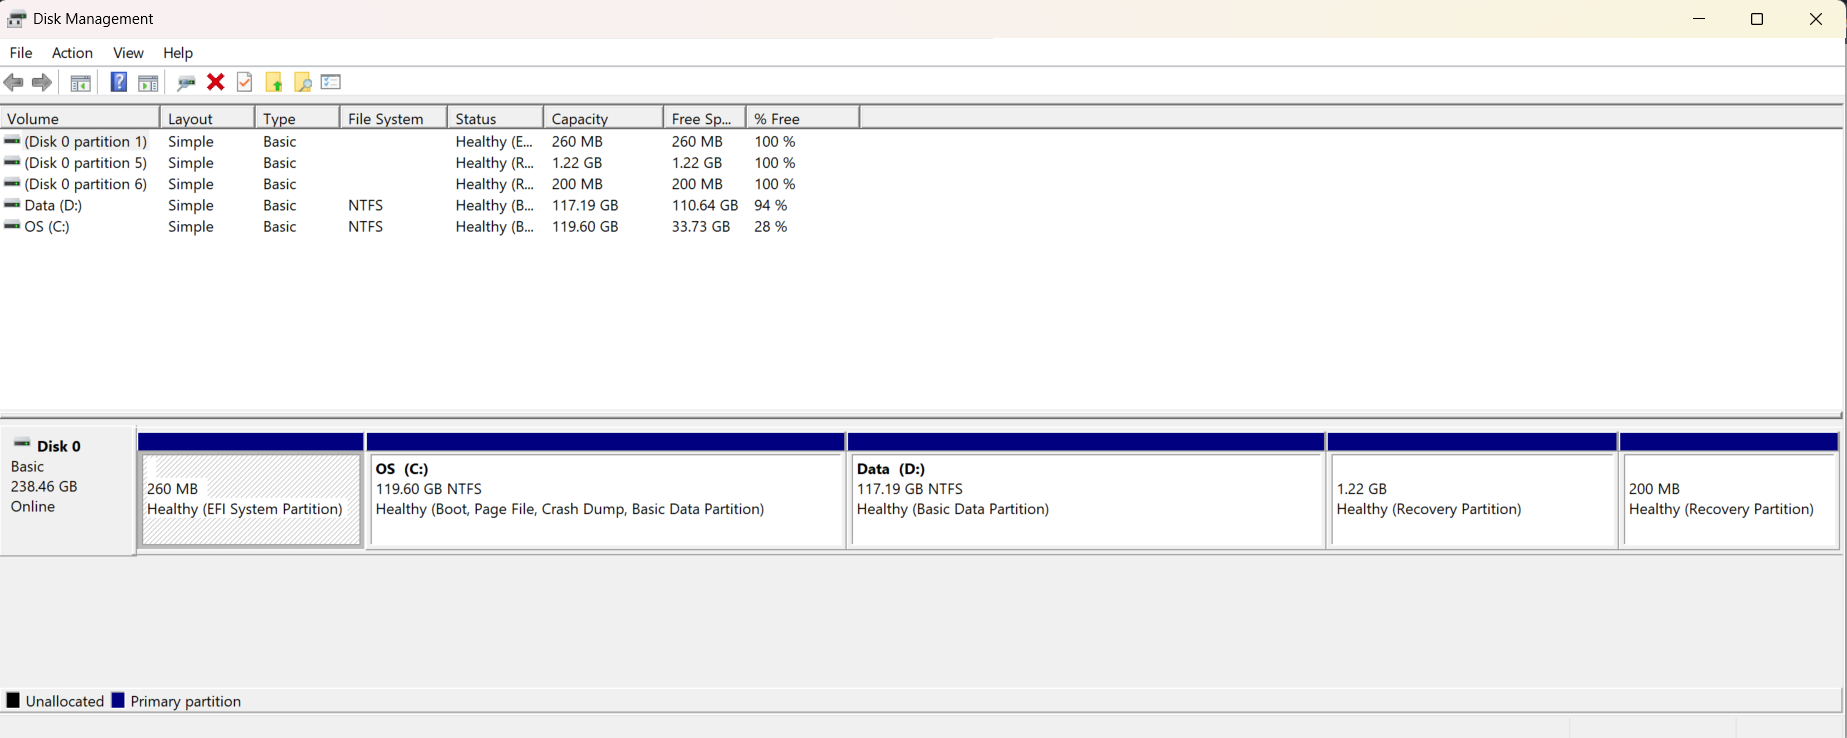
\includegraphics[width=0.9\textwidth]{Images/Stats/Disk.png}
    \caption{Giao diện chương trình Disk Management}
    \label{fig:cpu-z-disk}
\end{figure}

% --- Các thiết bị vào ra ---
\noindent\textbf{\large Các thiết bị vào ra:} (Thông số chi tiết thể hiện ở Hình \ref{fig:cpu-z-device})

\begin{itemize}
        \item \textbf{Thiết bị âm thanh (Audio inputs and outputs):} 
        \begin{itemize}
            \item \textbf{Microphone:} Realtek(R) Audio: microphone tích hợp.
            \item \textbf{Speakers:} Realtek(R) Audio: loa tích hợp laptop.
        \end{itemize}
        \item \textbf{Thiết bị nhập liệu giao tiếp người dùng (Human Interface Devices):} 
        \begin{itemize}
            \item \textbf{ASUS Precision Touchpad:} touchpad của laptop ASUS.
            \item \textbf{Nhiều thiết bị HID-compliant khác (chuột, bàn di, điều khiển hệ thống, v.v.):} các thiết bị phụ trợ nhập liệu như chuột rời, touchpad, bàn phím rời, các nút multimedia...
        \end{itemize}
        \item \textbf{Bàn phím (Keyboards):}
        \begin{itemize}
            \item \textbf{3 thiết bị HID Keyboard Device:} bàn phím laptop + bàn phím ảo + bàn phím rời.
            \item \textbf{PC/AT Enhanced PS/2 Keyboard (101/102-Key):} bàn phím vật lý mặc định gắn với mainboard qua cổng PS/2 hoặc emulated PS/2.
        \end{itemize}
        \item \textbf{Chuột và các thiết bị trỏ khác (Mice and other pointing devices):}
        \begin{itemize}
            \item \textbf{3 thiết bị HID-compliant mouse:} touchpad, chuột ngoài, hoặc thiết bị trỏ phụ (ví dụ: trackpoint, bút stylus...).
        \end{itemize}
    \end{itemize}

\begin{center}
    \fbox{\parbox{0.9\textwidth}{
        \centering
        \large Laptop đang sử dụng đa dạng và hiệu quả các thiết bị vào ra, từ đó mang lại trải nghiệm sử dụng tốt nhất cho người dùng.
    }}
\end{center}

\begin{figure}[H]
    \centering
    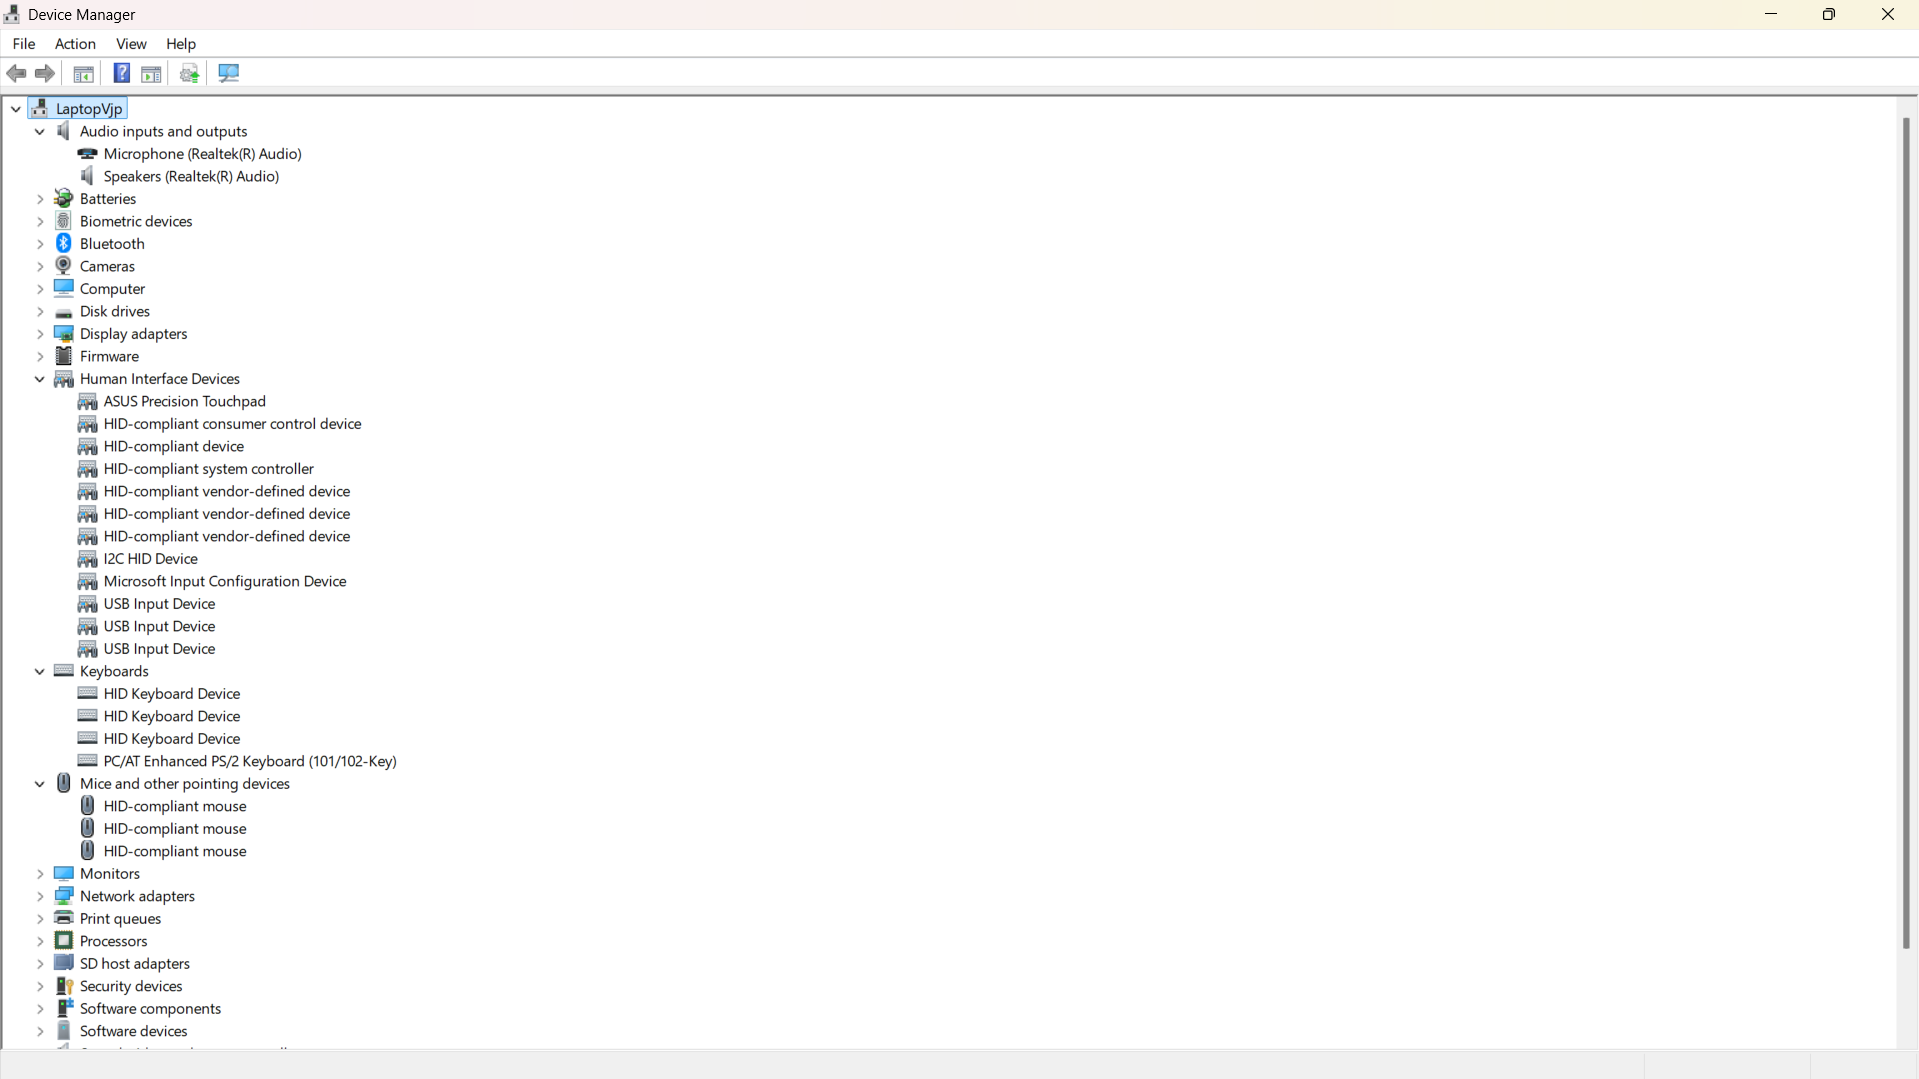
\includegraphics[width=1\textwidth]{Images/Stats/Device.png}
    \caption{Giao diện chương trình Device Manager}
    \label{fig:cpu-z-device}
\end{figure}

% --- Subtask 2 ---
\subsubsection{\textit{Dùng công cụ Debug khảo sát nội dung các thanh ghi IP, DS, ES, SS, CS, BP, SP}}

\noindent\textbf{\large Phần mềm khảo sát:} 
\begin{itemize}
    \item Sử dụng phần mềm emu8086 microprocessor emulator
\end{itemize}

\vspace{0.3cm}

\noindent\textbf{\large Các bước thực hiện:} 
\begin{itemize}
    \item Mở file .asm bằng phần mềm trên
    \item Chọn emulate trên thanh công cụ rồi chọn nút debug nằm cuối của cửa sổ vừa mở ra 
    \item Chạy Single step để xem kết quả debug từng mã lệnh từ đầu đến cuối
\end{itemize}

\vspace{0.3cm}

\noindent\textbf{\large Các kết quả khi chạy single step:} Kết quả chi tiết thể hiện ở các bước trong Hình \ref{fig:debug-steps}

\begin{figure}[H]
    \centering
    \begin{subfigure}[b]{0.48\textwidth}
        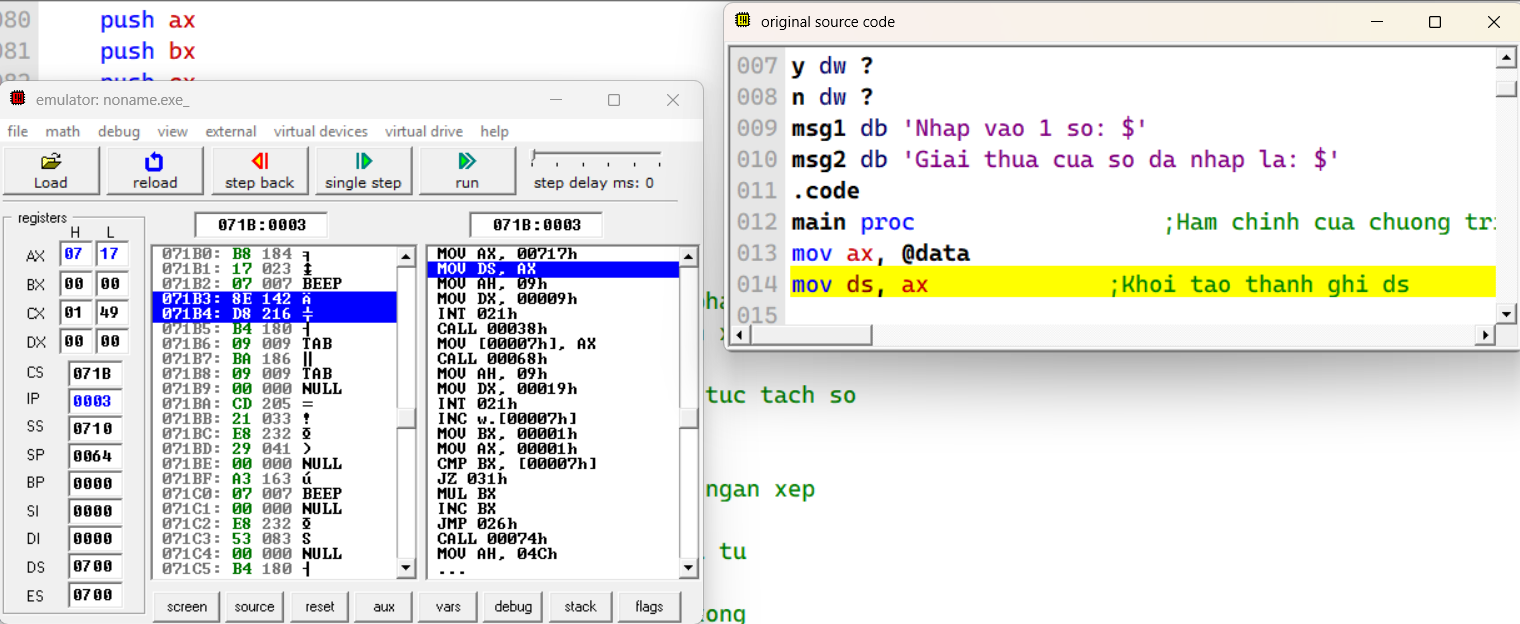
\includegraphics[width=\textwidth]{Images/Step/Step1.png}
        \caption{Bước 1}
    \end{subfigure}
    \hfill
    \begin{subfigure}[b]{0.48\textwidth}
        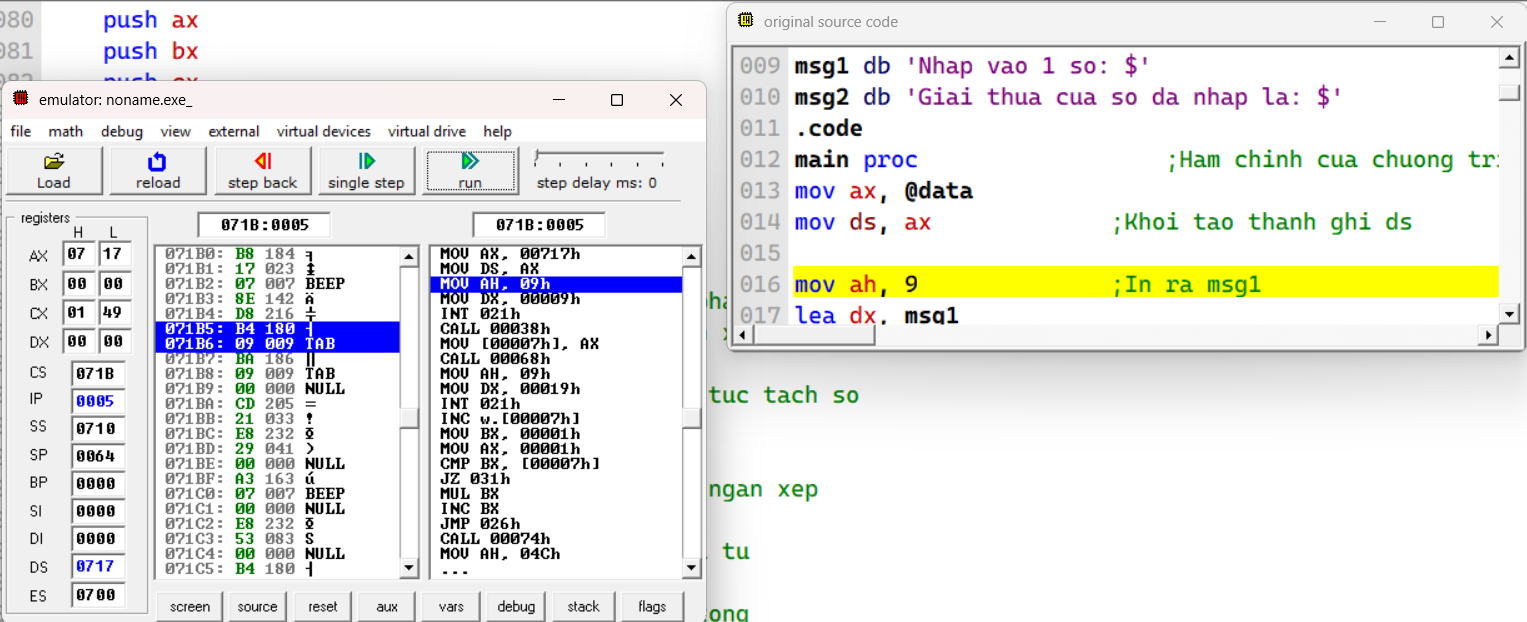
\includegraphics[width=\textwidth]{Images/Step/Step2.png}
        \caption{Bước 2}
    \end{subfigure}
    
    \vspace{0.5cm}
    
    \begin{subfigure}[b]{0.48\textwidth}
        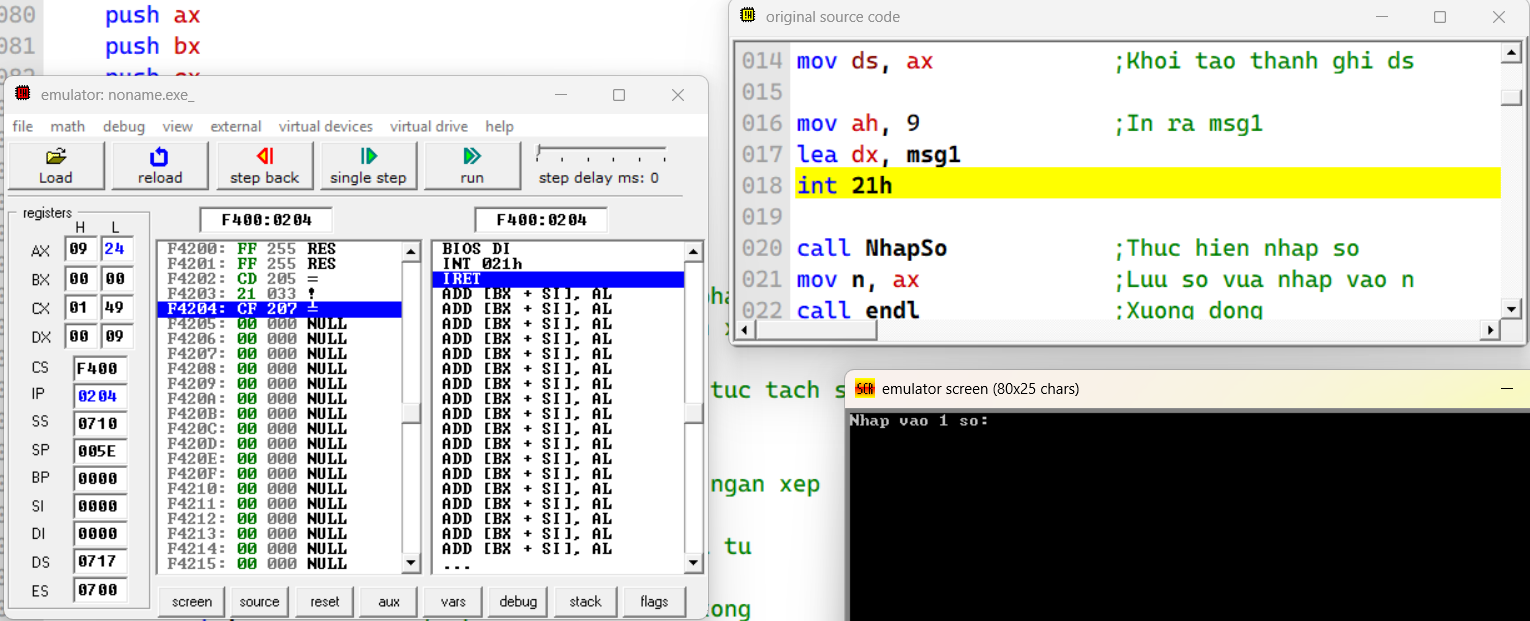
\includegraphics[width=\textwidth]{Images/Step/Step3.png}
        \caption{Bước 3}
    \end{subfigure}
    \hfill
    \begin{subfigure}[b]{0.48\textwidth}
        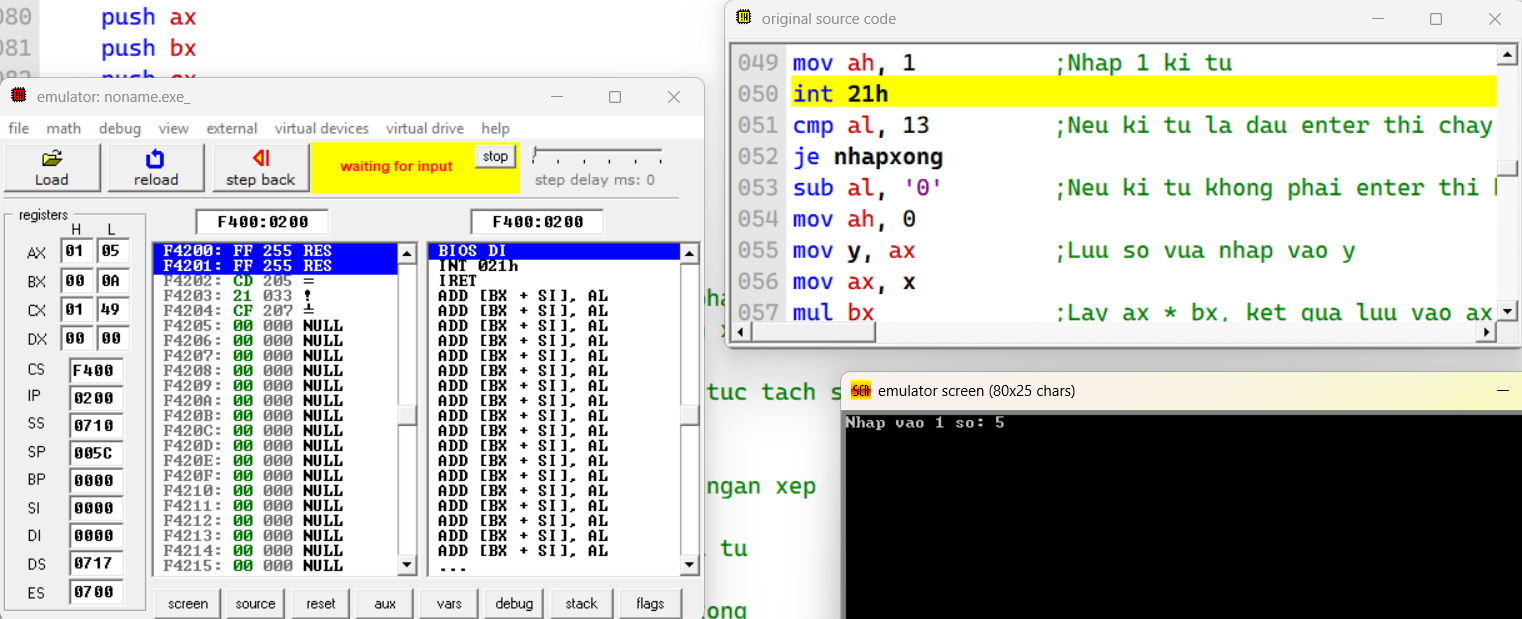
\includegraphics[width=\textwidth]{Images/Step/Step4.png}
        \caption{Bước 4}
    \end{subfigure}
    
    \vspace{0.5cm}
    
    \begin{subfigure}[b]{0.48\textwidth}
        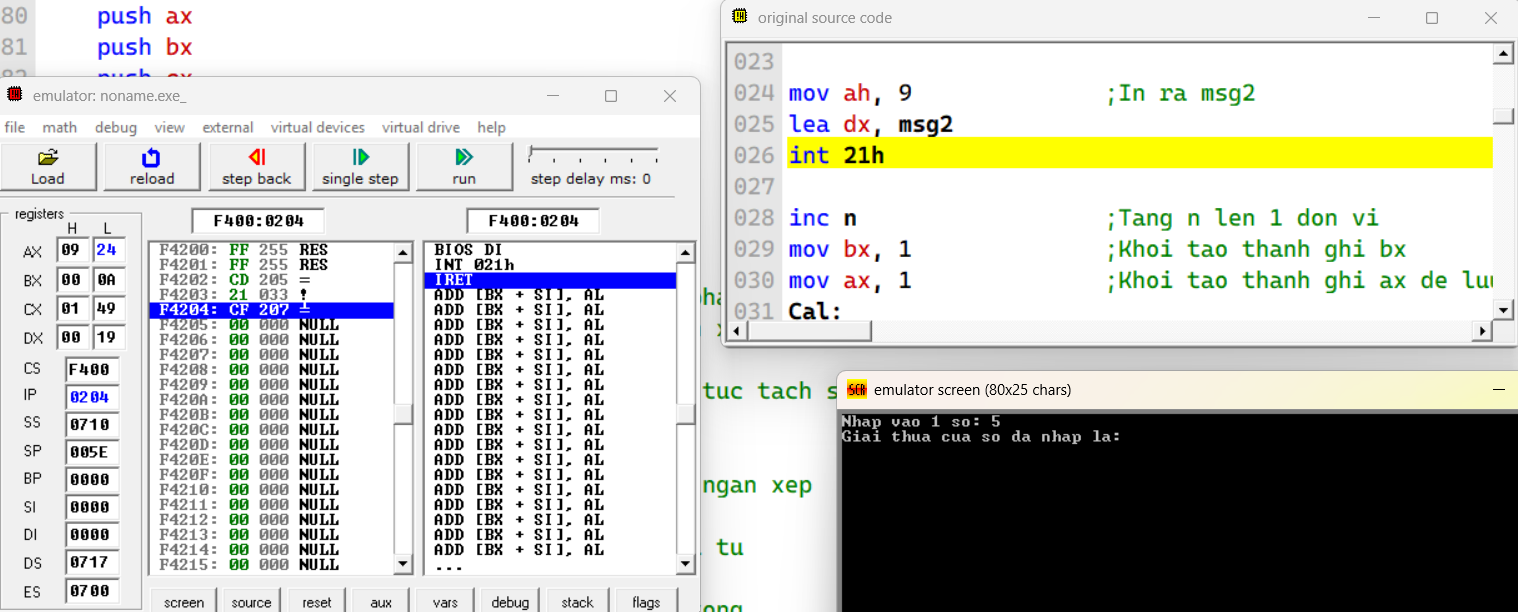
\includegraphics[width=\textwidth]{Images/Step/Step5.png}
        \caption{Bước 5}
    \end{subfigure}
    \hfill
    \begin{subfigure}[b]{0.48\textwidth}
        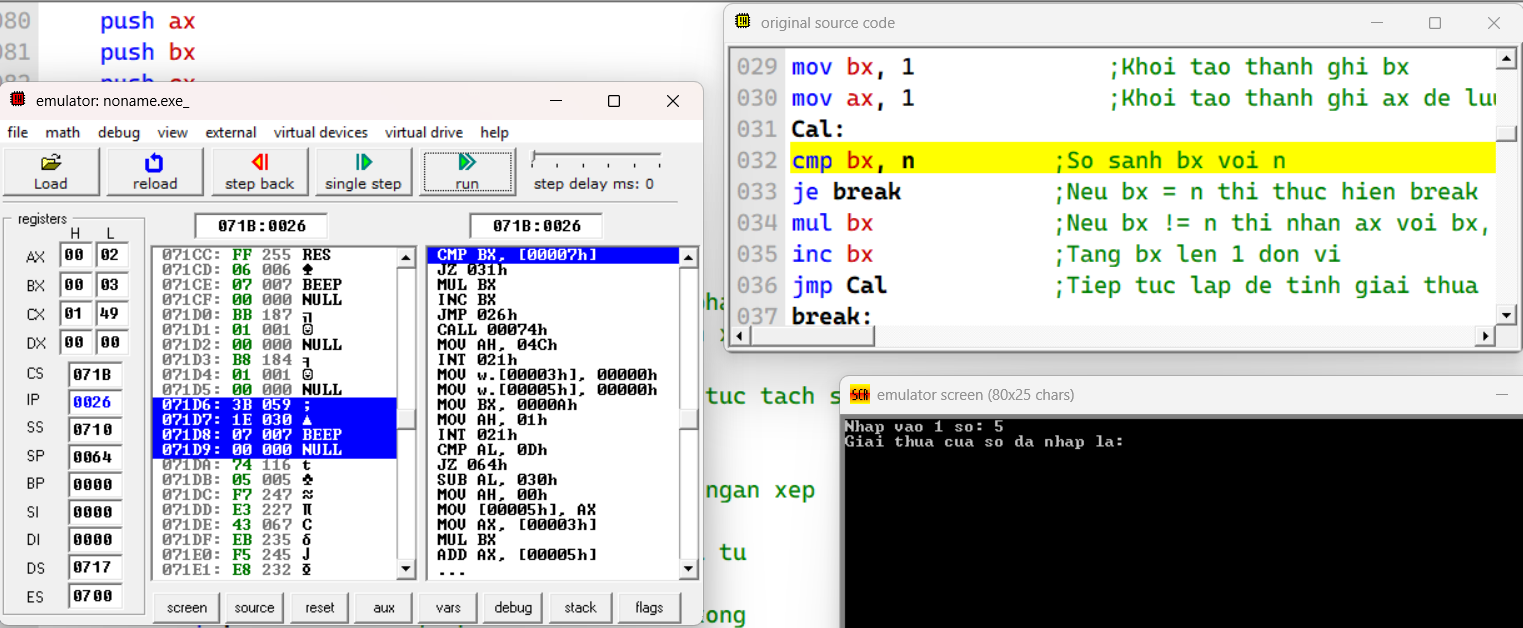
\includegraphics[width=\textwidth]{Images/Step/Step6.png}
        \caption{Bước 6}
    \end{subfigure}
    
    \vspace{0.5cm}
    
    \begin{subfigure}[b]{0.48\textwidth}
        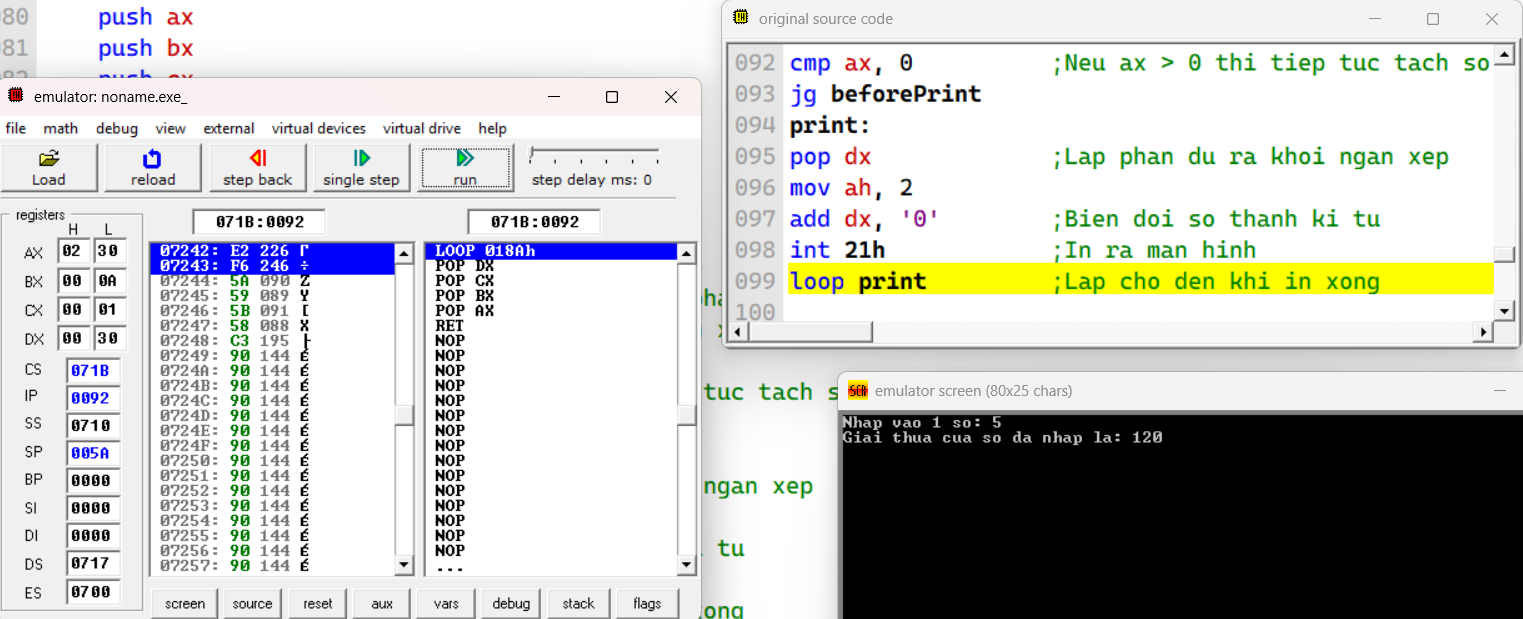
\includegraphics[width=\textwidth]{Images/Step/Step7.png}
        \caption{Bước 7}
    \end{subfigure}
    \hfill
    \begin{subfigure}[b]{0.48\textwidth}
        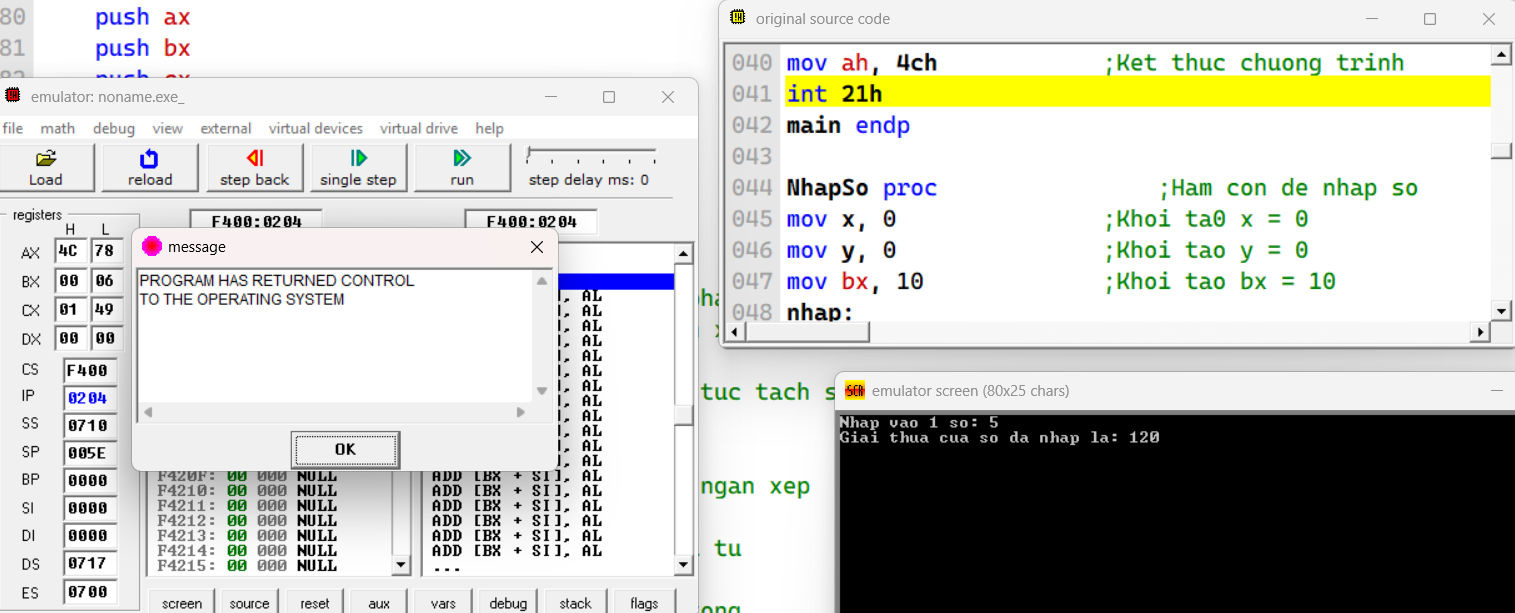
\includegraphics[width=\textwidth]{Images/Step/Step8.png}
        \caption{Bước 8}
    \end{subfigure}
    
    \caption{Các bước chạy single step khảo sát nội dung các thanh ghi.}
    \label{fig:debug-steps}
\end{figure}

% --- Subtask 3 ---
\subsubsection{\textit{Giải thích nội dung các thanh ghi, trên cơ sở đó giải thích cơ chế quản lý bộ nhớ của hệ thống trong trường hợp cụ thể.}}

\vspace{0.4cm}

\noindent\large 
Khi chương trình bắt đầu chạy, hệ điều hành tự động khởi tạo các thanh ghi, vùng nhớ và cấp phát không gian địa chỉ cho chương trình.

\vspace{0.4cm}

\noindent\large 
Tương ứng với các câu lệnh trong mã nguồn, nội dung các thanh ghi có thể thay đổi hoặc không.

\vspace{0.5cm}

\begin{itemize}
    \item \textbf{IP (Instruction Pointer):}
    \begin{itemize}
        \item \textbf{IP} là thanh ghi trỏ đến địa chỉ của lệnh tiếp theo sẽ được thực thi trong mã máy.
        \item Khi một chương trình được thực thi, \textbf{IP} được cập nhật để trỏ đến lệnh tiếp theo trong mã nguồn, giúp CPU biết lệnh nào sẽ được thực thi tiếp theo.
    \end{itemize}

    \item \textbf{DS (Data Segment) và SI (Source Index):}
    \begin{itemize}
        \item \textbf{DS} là thanh ghi chỉ đến phân đoạn dữ liệu, nơi dữ liệu chương trình được lưu trữ.
        \item \textbf{SI} thường được sử dụng trong các phép toán dữ liệu và là một trong các thanh ghi chỉ địa chỉ.
        \item Khi chương trình yêu cầu truy cập dữ liệu từ bộ nhớ, \textbf{DS} và \textbf{SI} thường được sử dụng để xác định vị trí của dữ liệu.
    \end{itemize}

    \item \textbf{SS (Stack Segment) và BP (Base Pointer):}
    \begin{itemize}
        \item \textbf{SS} là thanh ghi chỉ đến phân đoạn ngăn xếp (stack segment), nơi lưu trữ các giá trị cục bộ và địa chỉ của các hàm.
        \item \textbf{BP} thường được sử dụng để trỏ đến địa chỉ cơ sở của ngăn xếp (base of stack).
        \item Ngăn xếp được sử dụng để lưu trữ giá trị trung gian và địa chỉ trả về từ các hàm con trong quá trình thực thi chương trình.
    \end{itemize}

    \item \textbf{SP (Stack Pointer):}
    \begin{itemize}
        \item \textbf{SP} là thanh ghi chỉ đến đỉnh của ngăn xếp (top of stack).
        \item Khi dữ liệu được đẩy (push) hoặc rút (pop) ra khỏi ngăn xếp, \textbf{SP} sẽ thay đổi để chỉ đến vị trí mới nhất trong ngăn xếp.
        \item \textbf{SP} cũng được sử dụng để cấp phát không gian mới cho dữ liệu trong ngăn xếp.
    \end{itemize}
\end{itemize}

\vspace{0.6cm}

\noindent\large 
Cụ thể, trong trường hợp chương trình Assembly cho phép nhập vào một số và in ra màn hình giai thừa của số đó, cơ chế quản lý bộ nhớ như sau:

\vspace{0.5cm}

\begin{itemize}
    \item \textbf{Khởi tạo bộ nhớ:}
    \begin{itemize}
        \item Khi chương trình bắt đầu, hệ điều hành cấp phát các đoạn mã (code), dữ liệu (data) và ngăn xếp (stack) cho chương trình.
        \item Đoạn mã chứa các lệnh chương trình, đoạn dữ liệu chứa các biến, và ngăn xếp dùng để lưu trữ dữ liệu tạm thời.
    \end{itemize}

    \item \textbf{Phân đoạn bộ nhớ:}
    \begin{itemize}
        \item \textbf{CS} (Code Segment) trỏ tới đoạn mã của chương trình.
        \item \textbf{DS} (Data Segment) trỏ tới đoạn dữ liệu của chương trình.
        \item \textbf{SS} (Stack Segment) trỏ tới đoạn ngăn xếp của chương trình.
    \end{itemize}

    \item \textbf{Quản lý ngăn xếp:}
    \begin{itemize}
        \item Ngăn xếp được sử dụng để lưu trữ tạm thời dữ liệu và địa chỉ trả về khi gọi hàm.
        \item \textbf{SP} được khởi tạo với giá trị từ khai báo \texttt{.Stack 100}, nghĩa là kích thước ngăn xếp là 100 byte.
    \end{itemize}
\end{itemize}

\vspace{0.6cm}

\noindent\large 
Diễn giải nội dung của các câu lệnh trong mã nguồn và ảnh hưởng đến các thanh ghi:

\vspace{0.5cm}

\begin{itemize}
    \item \textbf{Khởi tạo đoạn dữ liệu:}
    \begin{lstlisting}[style=asm]
    mov ax, @data
    mov ds, ax  
    \end{lstlisting}
    \textbf{DS} trỏ tới đoạn dữ liệu, \textbf{AX} làm trung gian để chuyển địa chỉ đoạn dữ liệu vào \textbf{DS}.

    \item \textbf{Hiển thị thông báo:}
    \begin{lstlisting}[style=asm]
    mov ah, 9              
    lea dx, msg1
    int 21h
    \end{lstlisting}
    hoặc
    \begin{lstlisting}[style=asm]
    mov ah, 9              
    lea dx, msg2
    int 21h
    \end{lstlisting}
    Gắn \textbf{AH} = 9, \textbf{DX} trỏ tới địa chỉ chuỗi thông báo cần in ra màn hình.

    \item \textbf{Nhập dữ liệu:}
    Gọi hàm nhập số:
    \begin{lstlisting}[style=asm]
    call NhapSo 
    \end{lstlisting}
    Trong hàm \texttt{NhapSo}:
    \begin{lstlisting}[style=asm]
    NhapSo proc                
    mov x, 0               
    mov y, 0               
    mov bx, 10             
    nhap:   
        mov ah, 1         
        int 21h 
        cmp al, 13         
        je nhapxong
        sub al, '0'        
        mov ah, 0
        mov y, ax         
        mov ax, x
        mul bx            
        add ax, y       
        mov x, ax          
        jmp nhap        
    nhapxong:
        mov ax, x          
    ret
    NhapSo endp 
    \end{lstlisting}
    \begin{itemize}
        \item Gắn \textbf{AH} = 1 để nhập ký tự từ bàn phím, ký tự nhập vào lưu trong \textbf{AL}.
        \item Sau khi nhập xong, số nhập được gán vào thanh ghi \textbf{AX}.
    \end{itemize}

    \item \textbf{Tính giai thừa:}
    \begin{lstlisting}[style=asm]
    inc n                  
    mov bx, 1              
    mov ax, 1     
    Cal:
        cmp bx, n          
        je break           
        mul bx            
        inc bx           
        jmp Cal     
    \end{lstlisting}
    \textbf{AX} lưu kết quả phép nhân, \textbf{BX} lưu biến đếm sử dụng trong nhãn \texttt{Cal}.

    \item \textbf{In ra màn hình:}
    Gọi hàm in số:
    \begin{lstlisting}[style=asm]
    call InSo 
    \end{lstlisting}
    Trong hàm \texttt{InSo}:
    \begin{lstlisting}[style=asm]
    InSo proc                 
    push ax
    push bx
    push cx
    push dx
    
    mov bx, 10             
    mov cx, 0
    beforePrint:
        mov dx, 0
        div bx            
        push dx           
        inc cx          
        cmp ax, 0          
        jg beforePrint
    print:
        pop dx      
        mov ah, 2          
        add dx, '0'      
        int 21h      
        loop print       
    
    pop dx
    pop cx
    pop bx
    pop ax
    ret
    InSo endp
    \end{lstlisting}
    \begin{itemize}
        \item Đẩy \textbf{AX}, \textbf{BX}, \textbf{CX}, \textbf{DX} vào ngăn xếp để bảo vệ dữ liệu.
        \item Phân tách từng chữ số từ \textbf{AX} đưa vào stack, rồi lần lượt lấy ra in ra màn hình.
    \end{itemize}
\end{itemize}



\section{Phần làm nhóm}
\subsection{Giới thiệu đề tài}
Trò chơi \textit{Snake} (hay còn gọi là \textbf{rắn săn mồi}) là một trò chơi điện tử đơn giản nhưng kinh điển. Với lối chơi dễ hiểu nhưng đầy thử thách, Snake thường được lựa chọn làm bài tập thực hành trong các môn học về lập trình hoặc hệ thống máy tính. 

\vspace{0.5em}

Trong khuôn khổ môn học \textbf{Kiến trúc máy tính}, nhóm chúng em thực hiện đề tài xây dựng trò chơi Snake bằng ngôn ngữ Assembly trên trình giả lập \textbf{emu8086} - một môi trường mô phỏng vi xử lý Intel 8086 giúp người học tiếp cận sâu hơn với kiến trúc phần cứng và cách thức vận hành của một hệ thống máy tính ở mức thấp.

\vspace{0.5em}

\textbf{Mục tiêu đề tài:} Triển khai thành công trò chơi Snake với đầy đủ chức năng cơ bản như: điều khiển rắn bằng phím, sinh mồi ngẫu nhiên,... Ngoài ra, đề tài còn hướng tới việc khai thác hiệu quả các dịch vụ hệ thống qua ngắt BIOS/DOS (như \texttt{INT 10h}, \texttt{INT 16h}), từ đó nâng cao kỹ năng lập trình Assembly, hiểu rõ hơn về hoạt động của CPU, bộ nhớ, và giao tiếp phần cứng.

\vspace{0.5em}

\textbf{Giới hạn đề tài:} Đề tài giới hạn ở môi trường \textbf{chế độ văn bản} trên giả lập emu8086, không sử dụng đồ họa bitmap hay chế độ đồ họa nâng cao. Tốc độ xử lý và di chuyển của rắn được điều chỉnh bằng kỹ thuật trễ đơn giản, không sử dụng đa luồng hay xử lý song song. Tất cả logic trò chơi đều được viết thủ công bằng Assembly, không sử dụng thư viện hỗ trợ bên ngoài.

\vspace{0.5em}

\textbf{Nội dung báo cáo:} Dưới đây, chúng em:
\begin{itemize}
    \item \textbf{Phạm Tùng Dương}: làm phần 1 (in ra \texttt{msgstart}, \texttt{msgover}, viết các hàm \texttt{wait\_for\_enter}, \texttt{randomizeMeal} và nhãn \texttt{game\_over}).
    \item \textbf{Triệu Tuấn Anh}: làm phần 2 (làm nhãn \texttt{game\_loop} và các nhãn nằm trong \texttt{game\_loop}).
    \item \textbf{Lê Huy Đức}: làm phần 3 (các hàm \texttt{shownewhead}, \texttt{move\_snake} và \texttt{score\_plus}).
\end{itemize}
xin phép được trình bày về đề tài \textbf{Lập trình Snake Game trên Emu8086}

\subsection{Nội dung tổng quan về đề tài}
\begin{enumerate}[leftmargin=*, label=\textbf{\arabic*.}, itemsep=1em]
    
    \item \textbf{Nội dung chính}
    
    \vspace{0.3cm}
    \noindent\hangindent=1cm \hangafter=1
    Xây dựng trò chơi \textbf{Snake (rắn săn mồi)} bằng ngôn ngữ Assembly trên trình giả lập \textbf{Emu8086}. Trò chơi mô phỏng cơ chế rắn di chuyển, ăn mồi và phát triển độ dài, đồng thời xử lý va chạm với tường hoặc chính thân rắn để xác định điều kiện kết thúc.
    
    \item \textbf{Tổng quan về trò chơi}
    
    \begin{itemize}[leftmargin=1.5em, label=$\bullet$]
        \item Snake là trò chơi một người chơi, trong đó người chơi điều khiển một con rắn di chuyển liên tục trên màn hình để tìm và ăn các mồi xuất hiện ngẫu nhiên.
        
        \item Mỗi khi ăn được mồi, rắn sẽ dài ra và điểm số tăng lên.
        
        \item Trò chơi kết thúc khi rắn đâm vào chính thân mình.
        
        \item \textbf{Cách chơi:}
        \begin{itemize}[leftmargin=1.5em, label=$\circ$]
            \item Điều khiển bằng các phím mũi tên: ↑ ↓ ← →
            \item Rắn di chuyển tự động theo hướng hiện tại
            \item Không được quay ngược 180° tức thời
            \item Ăn mồi để tăng độ dài và điểm số
        \end{itemize}
        
        \item \textbf{Các chức năng chính:}
        \begin{itemize}[leftmargin=1.5em, label=$\circ$]
            \item Khởi tạo màn hình và vị trí ban đầu
            \item Sinh mồi ngẫu nhiên không trùng rắn
            \item Cập nhật chuyển động theo điều khiển
            \item Kiểm tra va chạm thân/tường
            \item Hiển thị điểm số khi kết thúc
        \end{itemize}
    \end{itemize}

    \item \textbf{Giải thuật và kỹ thuật}
    
    \begin{itemize}[leftmargin=1.5em, label=$\bullet$]
        \item \textbf{Cấu trúc dữ liệu:}
        \begin{itemize}[leftmargin=1.5em, label=$\circ$]
            \item Mảng tọa độ các đoạn thân rắn
            \item Vị trí mồi sinh ngẫu nhiên
        \end{itemize}
        
        \item \textbf{Thuật toán chính:}
        \begin{itemize}[leftmargin=1.5em, label=$\circ$]
            \item Di chuyển: đầu tiến, đuôi xóa (trừ khi ăn mồi)
            \item Kiểm tra trùng mồi để tăng điểm
            \item Phát hiện va chạm thân/tường
        \end{itemize}
        
        \item \textbf{Kỹ thuật xử lý:}
        \begin{itemize}[leftmargin=1.5em, label=$\circ$]
            \item Ngắt \texttt{INT 10h} để vẽ màn hình
            \item Ngắt \texttt{INT 16h} đọc phím
            \item Vòng lặp điều khiển rắn 
        \end{itemize}
    \end{itemize}
\end{enumerate}

\subsection{Phân tích chương trình}
\subsubsection{\textit{Lưu đồ thuật toán (Flowchart)}}

\vspace{0.5cm}
\noindent\textbf{\Large Flowchart của thuật toán:} Hình~\ref{fig:flowchart-group}

\vspace{0.3cm}
\begin{figure}[H]
    \centering
    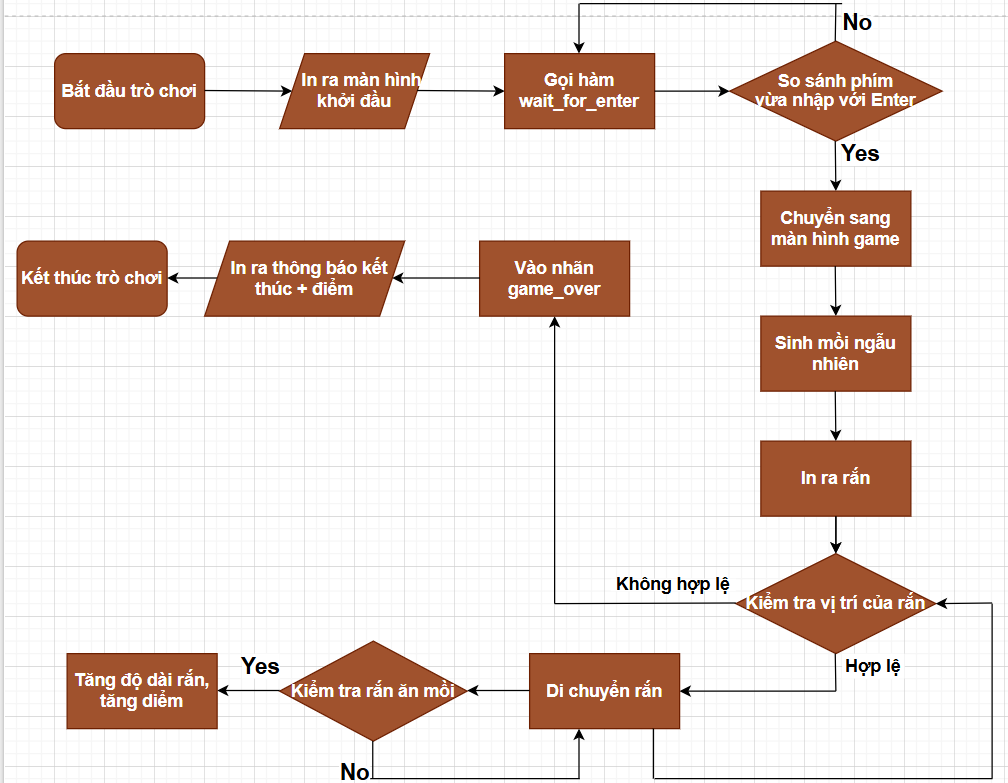
\includegraphics[width=0.9\textwidth]{Images/Flowchart/Flowchart-group.png}
    \caption{Flowchart Snake Game}
    \label{fig:flowchart-group}
\end{figure}

\vspace{0.4cm}
\noindent \textbf{Trong đó:}
\begin{itemize}
    \itemsep0.2cm
    \item \textbf{Dữ liệu đầu vào:} Người dùng nhập phím \texttt{\textbf{Enter}} để bắt đầu trò chơi, sử dụng các phím mũi tên \texttt{\textbf{↑ ↓ ← →}} để điều khiển rắn di chuyển.
    \item \textbf{Dữ liệu đầu ra:} Khi bắt đầu, in ra tên trò chơi và thông báo yêu cầu người dùng nhập \texttt{\textbf{Enter}} để chơi. Khi kết thúc, in ra thông báo \texttt{\textbf{"Game Over"}} và điểm của người chơi.
\end{itemize}

\subsubsection{\textit{Phân tích chi tiết}}
\vspace{0.5cm}

\noindent \textbf{Mã nguồn chi tiết của thuật toán tại:} \href{http://bit.ly/3GG2OQN}{\texttt{\large http://bit.ly/3GG2OQN}}

\vspace{0.5cm}
\noindent\textbf{\Large Phân tích chương trình:}
\vspace{0.3cm}

\begin{lstlisting}[style=asm]
    .model small
    .stack 100h
    .data
        snake dw 10Dh, 10Ch, 10Bh, 10Ah, 150 dup(?) 
        s_size db 4,0     
        tail dw ?         
        
        left  equ 4Bh  
        right equ 4Dh   
        up    equ 48h
        down  equ 50h
    
        cur_dir db right  
        old_dir db right    
        
        mealX db ?
        mealY db ?
    
        score db '0','0','0','0','$' 
        
        ;2 bien msgstart va msgover nhu hinh duoi
    .code
\end{lstlisting}

\vspace{0.4cm}
\begin{figure}[H]
    \centering
    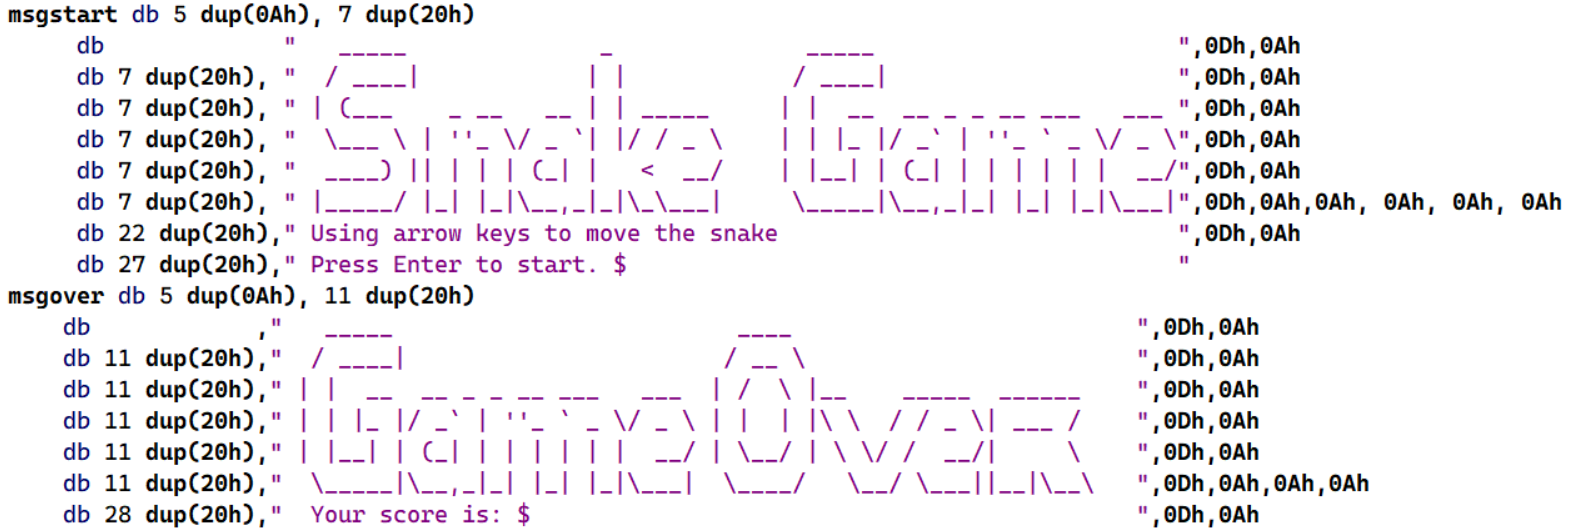
\includegraphics[width=0.9\textwidth]{Images/CodeSample/Code-1.png}
    \caption{Biến \texttt{msgstart} và \texttt{msgover}}
    \label{fig:codesample-1}
\end{figure}

\vspace{0.4cm}
\noindent \textbf{Trong đoạn code trên:}
\begin{itemize}
    \itemsep0.2cm
    \item \textbf{\texttt{.model small}}: chọn mô hình bộ nhớ "small", nghĩa là segment code và data riêng biệt, mỗi segment tối đa 64KB.
    \item \textbf{\texttt{.stack 100h}}: đặt vùng stack có kích thước 256 bytes (100h = 256).
    \item \textbf{\texttt{.data}}: bắt đầu khai báo biến.
    \item \textbf{\texttt{snake}}: khai báo con rắn ban đầu có 4 ô từ (10,1) đến (13,1), có 150 ô trống để thêm khi rắn ăn được mồi.
    \item \textbf{\texttt{s\_size}}: lưu độ dài rắn, ban đầu là 4.
    \item \textbf{\texttt{tail}}: lưu vị trí đuôi rắn.
    \item \textbf{\texttt{left, right, up, down}}: định nghĩa các biến ứng với phím mũi tên trên bàn phím.
    \item \textbf{\texttt{cur\_dir}}, \textbf{\texttt{old\_dir}}: lưu hướng hiện tại và hướng cũ của rắn, mặc định ban đầu là \texttt{right}.
    \item \textbf{\texttt{mealX}}, \textbf{\texttt{mealY}}: lưu tọa độ X, Y của mồi.
    \item \textbf{\texttt{score}}: lưu điểm của người chơi, tối đa 4 chữ số.
    \item \textbf{\texttt{msgstart}}: lưu nội dung màn hình bắt đầu.
    \item \textbf{\texttt{msgover}}: lưu nội dung khi trò chơi kết thúc.
\end{itemize}

\vspace{0.5cm}

\begin{lstlisting}[style=asm]
    main proc
    mov ax, @data
    mov ds, ax
                                     
    mov ah, 9   
    lea dx, msgstart                             
    int 21h  
                                    
    mov ax, 40h   
    mov es, ax    

    call wait_for_enter     

    mov al, 1     
    mov ah, 5      
    int 10h            
    
    call randomizeMeal
\end{lstlisting}

\vspace{0.4cm}
\noindent \textbf{Trong đoạn code trên:}
\begin{itemize}
    \itemsep0.2cm
    \item \textbf{\texttt{main proc}}: bắt đầu hàm main.
    \item \textbf{\texttt{mov ax, @data} | \texttt{mov ds, ax}}: dùng thanh ghi \texttt{ax} làm trung gian để gán các giá trị trong \texttt{.data} vào thanh ghi \texttt{ds}.
    \item \textbf{\texttt{mov ah, 9} | \texttt{lea dx, msgstart} | \texttt{int 21h}}: sử dụng ngắt 9 để in ra màn hình biến msgstart.
    \item \textbf{\texttt{mov ax, 40h} | \texttt{mov es, ax}}: dùng thanh ghi \texttt{ax} làm trung gian để gán \texttt{40h} cho \texttt{es}, nhằm lưu các thông số dòng, cột của màn hình trò chơi.
    \item \textbf{\texttt{call} \texttt{wait\_for\_enter}}: gọi hàm \texttt{wait\_for\_enter}, hàm này có nội dung như sau:
    
    \vspace{0.3cm}
    \begin{lstlisting}[style=asm]
        wait_for_enter proc
            push ax 
            wait_loop:
                mov ah, 0      
                int 16h        
                cmp al, 13      
                jne wait_loop  
            pop ax
            ret
        wait_for_enter endp  
    \end{lstlisting}
    \vspace{0.3cm}

    \begin{itemize}
        \item \textbf{\texttt{push ax}}: đẩy thanh ghi \texttt{ax} vào \texttt{stack} để bảo toàn dữ liệu.
        \item \textbf{\texttt{wait\_loop}}: vào nhãn \texttt{wait\_loop}
        \item \textbf{\texttt{mov ah, 0} | \texttt{int 16h}}: dùng ngắt 0 nhập kí tự, không in lên màn hình.
        \item \textbf{\texttt{cmp al, 13}}: so sánh kí tự vửa nhập với kí tự \texttt{Enter}.
        \item \textbf{\texttt{jne} \texttt{wait\_loop}}: nếu không phải là kí tự \texttt{Enter} thì tiếp tục lặp.
        \item \textbf{\texttt{pop ax} | \texttt{ret}}: trả lại giá trị cho thanh ghi \texttt{ax} và kết thúc hàm.
    \end{itemize}
    
    \item \textbf{\texttt{mov al, 1} | \texttt{mov ah, 5} | \texttt{int 10h}}: chuyển sang trang màn hình mới.
    \item \textbf{\texttt{call randomizeMeal}}: gọi hàm \texttt{randomizeMeal}, hàm này có nội dung như sau:
    
    \vspace{0.3cm}
    \begin{lstlisting}[style=asm]
        randomizeMeal proc
            mov ah, 00h  
            int 1ah      
                
            mov ax, dx     
            xor dx, dx     
            mov cx, 25      
            div cx         
            mov mealY, dl   
                
            mov ah, 00h    
            int 1ah 
                
            mov ax, dx      
            xor dx, dx
            mov cx, 80       
            div cx
            mov mealX, dl    
                
            mov dh, mealY      
            mov cx, w.s_size    
            xor bx, bx          
            
            check_snake:
                cmp dx, snake[bx]     
                je randomizeMeal      
                    
                add bx, 2             
                loop check_snake      
                
            mov ah, 02h         
            mov bh, 01h         
            int 10h
                
            mov al, 04h        
            mov bl, 0eh        
            mov cx, 1         
            mov ah, 09h        
            int 10h 
                
            ret
        randomizeMeal endp                              
    \end{lstlisting}
    \vspace{0.3cm}

    \begin{itemize}
        \item \textbf{\texttt{mov ah, 00h} | \texttt{int 1ah} | \texttt{mov ax, dx} | \texttt{xor dx, dx}}: lấy 1 giá trị ngẫu nhiên, dùng \texttt{dx} làm trung gian để lưu giá trị đó vào \texttt{ax}, sau đó gán lại \texttt{dx} = 0.
        \item \textbf{\texttt{mov cx, 25} | \texttt{div cx} | \texttt{mov mealY, dl}}: lấy giá trị ngẫu nhiên vừa có chia cho 25 (số dòng) rồi gán cho \texttt{mealY}.
        \item 7 dòng code tiếp theo: tương tự như \texttt{mealY}, tính và gán giá trị cho \texttt{mealX}.
        \item \textbf{\texttt{mov dh, mealY} | \texttt{mov cx, w.}\texttt{s\_size} | \texttt{xor bx, bx}}: gán tọa độ của mồi vào \texttt{dx}, chiều dài rắn vào \texttt{cx}, đưa \texttt{bx} về 0 để trỏ vào đoạn đầu của rắn.
        \item \textbf{\texttt{check\_snake}}: vào nhãn \texttt{check\_snake}.
        \item \textbf{\texttt{cmp dx, snake[bx]} | \texttt{je randomizeMeal}}: so sánh vị trí mồi với từng đoạn của rắn, nếu trùng nhau thì tạo lại mồi.
        \item \textbf{\texttt{add bx, 2} | \texttt{loop} \texttt{check\_snake}}: nếu không trùng nhau thì kiểm tra đến đoạn tiếp theo của con rắn.
        \item Các dòng code còn lại: in ra mồi trên màn hình.
    \end{itemize}

\begin{lstlisting}[style=asm]
    game_loop:
        call shownewhead
    
        mov dx, snake[0]     
        mov si, w.s_size    
        add si, w.s_size    
        sub si, 2            
        mov cx, w.s_size    
        sub cx, 4
        jz no_death          
    deathloop:              
        cmp dx, snake[si]    
        je game_over
        sub si, 2           
        dec cx               
        jnz deathloop        
    no_death:
        mov si, w.s_size     
        add si, w.s_size
        sub si, 2
        mov ax, snake[si]    
        mov tail, ax
    
        call move_snake             
    
        mov dx, snake[0]          
        mov al, mealX             
        mov ah, mealY
        cmp ax, dx                
        jne hide_old_tail         
        mov al, s_size            
        inc al
        mov s_size, al            
        mov ax, tail             
        mov bh, 0
        mov bl, s_size           
        add bl, s_size            
        sub bl, 2
        mov snake[bx], ax           
        call scoreplus              
        call randomizeMeal          
        jmp no_hide_old_tail       
    
    hide_old_tail:
        mov dx, tail            
        
        mov ah, 02h              
        int 10h
    
        mov al, ' '              
        mov ah, 09h              
        mov bl, 0Fh
        mov cx, 1     
        int 10h  
        
    no_hide_old_tail:
        mov ah, 01h             
        int 16h
        jz no_key
    
        mov ah, 00h           
        int 16h                 
        cur_dir
        mov cur_dir, ah
    
    no_key:
        jmp game_loop           
\end{lstlisting}

\vspace{0.5cm}
\noindent \textbf{Trong đoạn code trên:}
\begin{itemize}
    \itemsep0.3cm
    \item \textbf{\texttt{call shownewhead}: gọi đến hàm \texttt{shownewhead} có nội dung như sau}:
    
    \vspace{0.3cm}
    \begin{lstlisting}[style=asm]
        shownewhead proc
            mov dx, snake[0]      
            
            mov ah, 02h        
            int 10h            
            
            mov al, 002        
            mov ah, 09h       
            mov bl, 0Ah
            mov bh, 01h
            mov cx, 1
            int 10h 
            
            ret
        shownewhead endp                          
    \end{lstlisting}
    \vspace{0.3cm}
    
    \begin{itemize}
        \itemsep0.2cm
        \item \textbf{\texttt{mov dx, snake[0]} | \texttt{mov ah, 02h} | \texttt{int 10h}}: lưu vị trí đoạn đầu của rắn vào \texttt{dx}, đồng thời di chuyển con trỏ đến vị trí đó.
        \item Các dòng code còn lại: hiển thị rắn lên màn hình (chiều dài mặc định là 4).
    \end{itemize}

    \item 5 dòng code tiếp theo: lưu độ dài của rắn và trỏ tới đuôi rắn.
    \item \textbf{\texttt{sub cx, 4} | \texttt{jz} \texttt{no\_death}}: Kiểm tra nếu độ dài rắn bằng 4 (độ dài mặc định) => rắn không thế chết, nhảy vào nhãn \texttt{no\_death}.
    \item \textbf{\texttt{deathloop}}: vào nhãn \texttt{deathloop}.
    \item \textbf{\texttt{cmp dx, snake[si]} | \texttt{je} \texttt{game\_over}}: Kiểm tra nếu đầu rắn và thân rắn trùng nhau => rắn chết, nhảy vào nhãn \texttt{game\_over}. Nhãn này có nội dung như sau:
    
    \vspace{0.3cm}
    \begin{lstlisting}[style=asm]
        game_over:
            xor dx, dx                      
            
            mov ah, 02h                   
            int 10h                  
            
            mov ah, 9                     
            lea dx, msgover  
            int 21h   
            
            mov ah, 9
            lea dx, score                   
            int 21h                   
    \end{lstlisting}
    \vspace{0.3cm}
    
    \begin{itemize}
        \itemsep0.2cm
        \item \textbf{\texttt{xor dx, dx}}: đặt lại \texttt{dx} = 0.
        \item \textbf{\texttt{mov ah, 02h} | \texttt{int 10h}}: đưa con trỏ về lại vị trí \texttt{dx}.
        \item Các dòng còn lại: in ra màn hình thông báo \texttt{Game Over} và điểm của người chơi.
    \end{itemize}

    \item 3 dòng tiếp theo: nếu không trùng nhau, nhảy đến các đoạn còn lại của rắn và tiếp tục kiểm tra.
    \item \textbf{\texttt{no\_death:}} vào nhãn \texttt{no\_death}.
    \item 5 dòng tiếp theo: xác định lại vị trí đuôi rắn (có thể bị thay đổi nếu nhảy vào \texttt{deathloop}), sau đó lưu vào \texttt{tail} qua thanh ghi \texttt{ax}.
    \item \textbf{\texttt{call} \texttt{move\_snake}}: vào hàm \texttt{move\_snake}. Hàm này có nội dung như sau:
    
    \vspace{0.3cm}
    \begin{lstlisting}[style=asm]
        move_snake proc
            mov di, w.s_size         
            add di, w.s_size
            sub di, 2
        
            mov cx, w.s_size         
            dec cx                   
        
            move_array:
                mov ax, snake[di-2]   
                mov snake[di], ax     
                sub di, 2            
                loop move_array       
            
            getdir:                     
                cmp cur_dir, left
                je move_left
                cmp cur_dir, right
                je move_right
                cmp cur_dir, up
                je move_up
                cmp cur_dir, down
                je move_down
            
            get_old_dir:               
                mov al, old_dir
                mov cur_dir, al
                jmp getdir 
                
            move_left:                   
                cmp old_dir, right      
                je get_old_dir
                mov al, b.snake[0]      
                dec al                   
                mov b.snake[0], al       
                cmp al, -1               
                stop_move
                jne stop_move            
                mov al, es:[4ah]         
                dec al                  
                mov b.snake[0], al       
                jmp stop_move            
            
            move_right:                  
                cmp old_dir, left
                je get_old_dir
                mov al, b.snake[0]
                inc al
                mov b.snake[0], al
                cmp al, es:[4ah]
                jb stop_move
                mov b.snake[0], 0
                jmp stop_move
             
            move_up:                    
                cmp old_dir, down
                je get_old_dir
                mov al, b.snake[1]
                dec al
                mov b.snake[1], al
                cmp al, -1
                jne stop_move
                mov al, es:[84h]
                mov b.snake[1], al
                jmp stop_move 
                
            move_down:                   
                cmp old_dir, up
                je get_old_dir
                mov al, b.snake[1]
                inc al
                mov b.snake[1], al
                cmp al, es:[84h]
                jbe stop_move
                mov b.snake[1], 0
                jmp stop_move
            
            stop_move:                       
                mov al, cur_dir
                mov old_dir, al
            ret
        move_snake endp            
    \end{lstlisting}
    \vspace{0.3cm}
    
    \begin{itemize}
        \itemsep0.2cm
        \item 4 dòng đầu: tính toán vị trí đuôi rắn và lưu vào \texttt{cx}.
        \item \textbf{\texttt{dec cx}}: giảm \texttt{cx} đi 1 đơn vị (sử dụng để đếm số vòng lặp).
        \item \textbf{\texttt{move\_array:}} vào nhãn \texttt{move\_array}. Nhãn này có nhiệm vụ lần lượt lưu vị trí trước đó của rắn vào ví trí tiếp theo (di chuyển rắn).
        \item \textbf{\texttt{getdir:}} vào nhãn \texttt{getdir}. Nhãn này sẽ kiểm tra hướng đi hiện tại, sau đó gọi vào các nhãn tương ứng.
        \item \textbf{\texttt{get\_old\_dir}}: vào nhãn \texttt{get\_old\_dir}. Nhãn này sẽ được vào nếu người chơi nhấn các phím khác ngoài phím mũi tên, khi đó rắn sẽ tiếp tục đi theo vị trí cũ.
        \item \textbf{\texttt{move\_left}}: vào nhãn \texttt{move\_left}.
        \item \textbf{\texttt{cmp} \texttt{old\_dir}\texttt{, right} | \texttt{je} \texttt{get\_old\_dir}}: nếu rắn đang sang phải, tiếp tục đi theo hướng cũ (vì rắn không thể quay 180°).
        \item 3 dòng tiếp theo: nếu rắn đang đi lên/xuống, trừ tọa độ x của đầu rắn đi 1 đơn vị (chuyển hướng rắn sang trái).
        \item \textbf{\texttt{cmp al, -1} | \texttt{jne} \texttt{stop\_move}}: nếu tọa độ đầu rắn vẫn còn ở trong màn hình thì vào nhãn \texttt{stop\_move}.
        \item 4 dòng tiếp theo: nếu tọa độ đầu rắn ra khỏi biên trái màn hình thì đưa đầu rắn sang biên bên phải (tạo hiệu ứng đi xuyên tường), rồi nhảy vào nhãn \texttt{stop\_move}.
        \item \textbf{\texttt{move\_right} | \texttt{move\_up} | \texttt{move\_down}}: các nhãn này có logic xử lí tương tự như nhãn \texttt{move\_left}.
        \item \textbf{\texttt{stop\_move}}: vào nhãn \texttt{stop\_move}. Nhãn này có nhiệm vụ lưu hướng đi hiện tại vào hướng đi cũ (được sử dụng khi người dùng nhấn trùng hướng di chuyển của rắn).
    \end{itemize}

    \item \textbf{\texttt{mov dx, snake[0]} | \texttt{mov al, mealX} | \texttt{mov ah, mealY}}: lưu tọa độ đầu rắn vào \texttt{dx}, tọa đồ mồi vào \texttt{ax}.
    \item \textbf{\texttt{cmp ax, dx} | \texttt{jne} \texttt{hide\_old\_tail}}: nếu tọa độ đầu rắn khác tọa độ mồi (rắn chưa ăn được mồi) thì vào nhãn \texttt{hide\_old\_tail}.
    \item 9 dòng tiếp theo: nếu rắn ăn được mồi thì tăng độ dài rắn, đồng thời thêm tọa độ đuôi mới cho rắn.
    \item \textbf{\texttt{call scoreplus} | \texttt{call randomizeMeal}}: gọi tới các hàm \texttt{randomizeMeal} để cập nhật mồi mới và \texttt{scoreplus} để cộng thêm điểm cho người chơi. Trong đó, hàm \texttt{scoreplus} có nội dung như sau: 
    
    \vspace{0.3cm}
    \begin{lstlisting}[style=asm]
        scoreplus proc
            mov al, score[3]             
            inc al                      
            cmp al, '9'                  
            jg inc_second
            mov score[3], al            
            ret
        
        inc_second:
            mov score[3], '0'            
            mov al, score[2]
            inc al
            cmp al, '9'
            jg inc_third
            mov score[2], al
            ret
        
        inc_third:                      
            mov score[2], '0'
            mov al, score[1]
            inc al
            cmp al, '9'
            jg inc_fourth
            mov score[1], al
            ret
        
        inc_fourth:                      
            mov score[1], '0'
            mov al, score[0]
            inc al
            mov score[0], al
            ret  
        scoreplus endp                                                                  
    \end{lstlisting}
    \vspace{0.3cm}
    
    \begin{itemize}
        \itemsep0.2cm
        \item \textbf{\texttt{mov al, score[3]} | \texttt{inc al}}: lưu số cuối vào \texttt{al}, đông thời tăng giá trị số đó lên 1 đơn vị (vì rắn vừa ăn được mồi).
        \item \textbf{\texttt{cmp al, }\texttt{'9'} | \texttt{jg} \texttt{inc\_second}}: so sánh số đó với 9, nếu lớn hơn thì vào nhãn \texttt{inc\_second}.
        \item \textbf{\texttt{mov score[3], al }}: nếu số nhỏ hơn 9 thì lưu kết quả và kết thúc hàm.
        \item \textbf{\texttt{inc\_second} | \texttt{inc\_third} | \texttt{inc\_fourth}}: các nhãn này có nội dung tương tự như phần trên, lần lượt cộng điểm cho số hàng chục, trăm và nghìn.
    \end{itemize}

\vspace{0.5cm}

\begin{lstlisting}[style=asm]
    mov ah, 4ch
    int 21h         
\end{lstlisting}

\vspace{0.5cm}
\noindent \textbf{Cuối cùng}, 2 dòng code trên được chạy ngay sau nhãn \texttt{game\_over} để kết thúc chương trình. 
\end{itemize}
\end{itemize}


\subsection{Kiểm tra giao diện chương trình}
\vspace{0.3cm}
\noindent Trong phần này, nhóm chúng em sẽ trình bày kết quả khi chạy chương trình:

\begin{figure}[H]
    \centering
    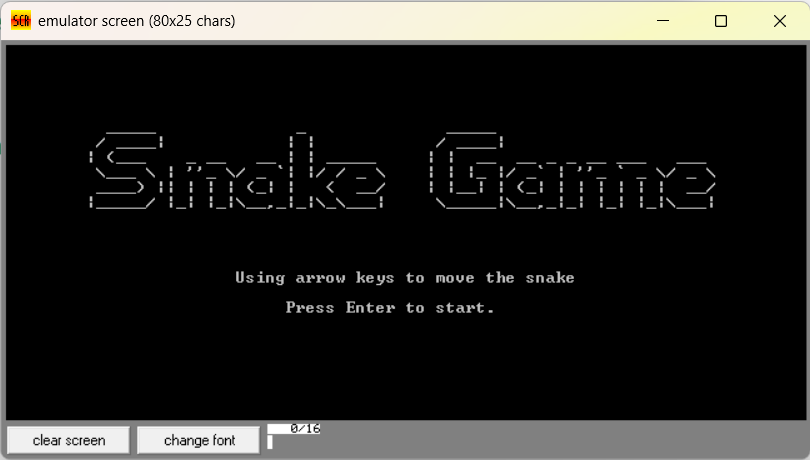
\includegraphics[width=0.85\textwidth]{Images/Game_Test/Game_test_1.png}
    \caption{Giao diện khởi đầu game}
    \label{fig:game_test_1}
\end{figure}

\noindent \textbf{Màn hình khởi đầu bao gồm:}
\begin{itemize}
    \itemsep0.2cm
    \item \textbf{Tiêu đề game:} Dòng chữ "Snake Game" được thiết kế bắt mắt.
    \item \textbf{Hướng dẫn:} Thông báo yêu cầu người chơi nhấn phím \texttt{Enter} để bắt đầu.
    \item \textbf{Tính năng:} Màn hình sẽ chuyển sang giao diện chính khi người dùng nhấn đúng phím \texttt{Enter}.
\end{itemize}

\vspace{0.5cm}
\begin{figure}[H]
    \centering
    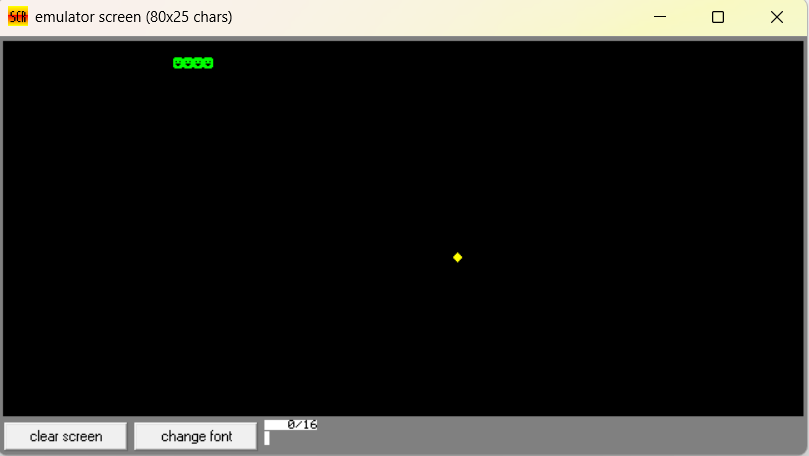
\includegraphics[width=0.85\textwidth]{Images/Game_Test/Game_test_2.png}
    \caption{Giao diện chính của game}
    \label{fig:game_test_2}
\end{figure}

\noindent \textbf{Giao diện chơi game bao gồm:}
\begin{itemize}
    \itemsep0.2cm
    \item \textbf{Con rắn:} 
    \begin{itemize}
        \item Độ dài ban đầu: 4 ô.
        \item Màu sắc mặc định: Xanh lá (\textcolor{green}{$\blacksquare$}).
    \end{itemize}
    \item \textbf{Mồi:}
    \begin{itemize}
        \item Kích thước: 1 ô.
        \item Màu sắc mặc định: Vàng (\textcolor{yellow}{$\blacksquare$}).
    \end{itemize}
    \item \textbf{Điều khiển:} Sử dụng các phím mũi tên ↑ ↓ ← → để di chuyển
\end{itemize}

\vspace{0.5cm}
\begin{figure}[H]
    \centering
    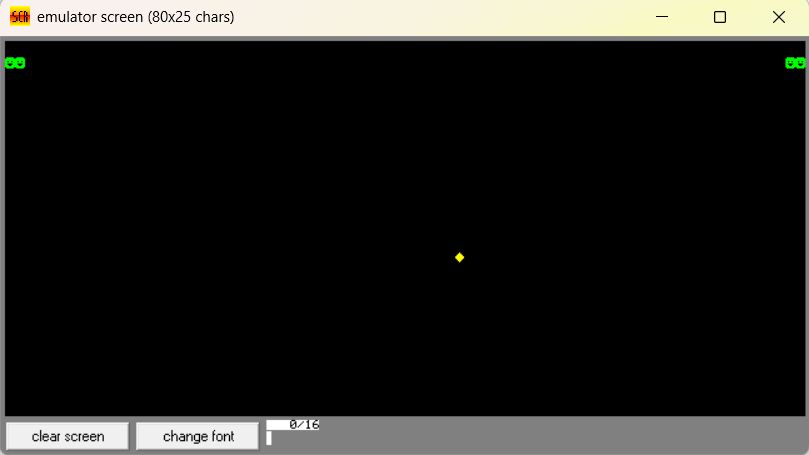
\includegraphics[width=0.85\textwidth]{Images/Game_Test/Game_test_3.png}
    \caption{Cơ chế xuyên tường}
    \label{fig:game_test_3}
\end{figure}

\noindent \textbf{Đặc điểm nổi bật:}
\begin{itemize}
    \itemsep0.2cm
    \item Khi rắn va chạm với tường, thay vì kết thúc game, rắn sẽ xuất hiện ở phía đối diện.
    \item Cơ chế này tạo độ khó vừa phải và tăng tính thú vị cho trò chơi.
\end{itemize}

\vspace{0.5cm}
\begin{figure}[H]
    \centering
    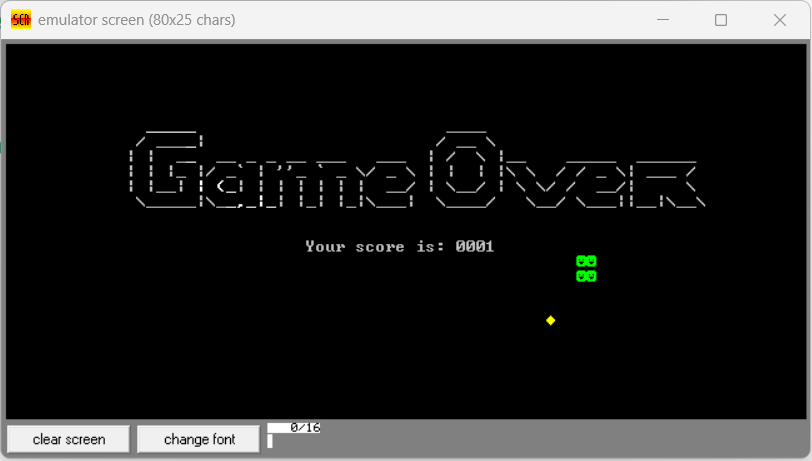
\includegraphics[width=0.85\textwidth]{Images/Game_Test/Game_test_4.png}
    \caption{Màn hình kết thúc game}
    \label{fig:game_test_4}
\end{figure}

\noindent \textbf{Màn hình kết thúc bao gồm:}
\begin{itemize}
    \itemsep0.2cm
    \item \textbf{Trạng thái cuối:} Vị trí rắn và mồi khi game kết thúc.
    \item \textbf{Thông báo:} Dòng chữ "Game Over" nổi bật.
    \item \textbf{Điểm số:} Hiển thị tổng điểm người chơi đạt được.
\end{itemize}

% --- Trang kết thúc ---
\newpage
\thispagestyle{empty}

\vspace*{2cm}

\begin{center}
    {\Huge \bfseries \textcolor{blue!60!black}{KẾT LUẬN}}\\[1cm]
    
    \rule{0.6\linewidth}{1pt}\\[1cm]

    \begin{tcolorbox}[colback=blue!5!white, colframe=blue!30!black,
        width=0.85\textwidth, sharp corners=south, boxrule=0.8pt,
        drop shadow southwest, enhanced, fonttitle=\bfseries]
        \Large
        Sau quá trình học tập và thực hiện, dự án đã hoàn thành với hai phần chính:\\ \textbf{(1)} ba bài tập cá nhân giúp củng cố kiến thức nền tảng\\ \textbf{(2)} bài tập nhóm là trò chơi \textit{Snake Game} được lập trình bằng ngôn ngữ Assembly, thể hiện sự phối hợp và vận dụng kỹ năng lập trình cấp thấp trong thực tiễn.

        \vspace{0.5cm}

        Dự án không chỉ giúp rèn luyện tư duy logic, kỹ năng xử lý sự kiện và quản lý bộ nhớ, mà còn nâng cao tinh thần làm việc nhóm, trách nhiệm và sáng tạo trong quá trình phát triển phần mềm.

        \vspace{0.5cm}

        Chúng em xin chân thành cảm ơn thầy đã hướng dẫn tận tình và tạo điều kiện để thực hiện bài tập lớn này.

        \vspace{0.5cm}

        Mọi góp ý và nhận xét từ thầy và các bạn sẽ là nguồn động lực để chúng em tiếp tục hoàn thiện kỹ năng trong học tập và công việc sau này.
    \end{tcolorbox}

    \vfill

    {\large \textit{Hà Nội, tháng 5 năm 2025}}

\end{center}


\end{document}
